% !TEX root = main.tex
% !TEX program = lualatex
% !BIB program = biber

% !TEX root = ../main.tex

% DO NOT TOUCH! unless absolutely necessary (consider updating the template then)

\documentclass[11pt, oneside]{book} % TODO add 'final' option once document is complete
\usepackage[a4paper,
            width=150mm,
            top=35mm,
            bottom=35mm,
            bindingoffset=10mm,
            marginparwidth=30mm,
            headheight=5mm,
            headsep=10mm,
            footskip=15mm,
            hcentering]{geometry}
\usepackage[backend=biber, sorting=nyt, citestyle=numeric-comp, bibstyle=ieee, maxbibnames=999]{biblatex}
\usepackage[ngerman, american]{babel}
\usepackage{setspace}
\usepackage{fancyhdr}
\usepackage[pdfusetitle, hidelinks]{hyperref}
\usepackage{mathtools}
\usepackage[warnings-off={mathtools-colon,mathtools-overbracket}]{unicode-math}
\usepackage{amsthm}
\usepackage{upgreek}
\usepackage{nicefrac}
\usepackage{algorithm}
\usepackage[beginComment=, beginLComment=, endLComment=]{algpseudocodex}
\usepackage{listings}
\usepackage{mleftright}
\usepackage{graphicx}
\usepackage{csquotes}
\usepackage{parskip}
\usepackage{titlesec}
\usepackage{xcolor}
\usepackage{lipsum}
\usepackage{pgfplots}
\usepackage{tikzpagenodes}
\usepackage{bookmark}
\usepackage{xurl}
\usepackage{etoolbox}
\usepackage{comment}
\usepackage{booktabs}
\usepackage{tabularx}
\usepackage{emptypage}
\usepackage{letltxmacro}
\usepackage[all]{nowidow}
\usepackage[final]{microtype}
\usepackage[nottoc]{tocbibind}
\usepackage[shortcuts]{extdash}
\usepackage[detect-all]{siunitx}
\usepackage[skip=5pt]{subcaption}
\usepackage[obeyFinal]{todonotes}
\usepackage[shortlabels]{enumitem}
\usepackage[nodayofweek]{datetime}
\usepackage{totcount}
\usepackage[figure,table,lstlisting,algorithm]{totalcount}
\usepackage[capitalize, nameinlink, noabbrev]{cleveref}
\usepackage[format=hang, font={color=darkgray, singlespacing}, skip=5pt]{caption}
\usepackage[lang-warn=false]{datatool-base}
\usepackage[style=alttree, acronym, symbols, nomain, nonumberlist, shortcuts=ac]{glossaries-extra}

% custom macros
% !TEX root = ../main.tex

% math typesetting utilities
\newcommand*{\given}{\;\middle|\;}
\newcommand*{\hateq}{\mathrel{\widehat{=}}}
\newcommand*{\tuple}[1]{\left\langle #1 \right\rangle}
\newcommand*{\set}[1]{\left\{ #1 \right\}}
\newcommand*{\multiset}[1]{\left\{\!\left\{ #1 \right\}\!\right\}}
\newcommand*{\evalat}[2][]{\left. #2 \right\rvert_{#1}}
\newcommand*{\bmat}[1]{\begin{bmatrix} #1 \end{bmatrix}}
\newcommand*{\sbmat}[1]{\begin{bsmallmatrix} #1 \end{bsmallmatrix}}
\newcommand*{\dbmat}[1]{\everymath{\displaystyle} \begin{bmatrix} #1 \end{bmatrix}}
\newcommand*{\abs}[1]{\left\lvert #1 \right\rvert}
\newcommand*{\norm}[1]{\left\lVert #1 \right\rVert}
\newcommand*{\bvec}[1]{{\symbfit{#1}}}

% math operators
\DeclareMathOperator*{\argmax}{arg\,max}
\DeclareMathOperator*{\argmin}{arg\,min}
\DeclareMathOperator*{\Exp}{\symbb{E}}
\DeclareMathOperator*{\Prob}{\symbb{P}}
\newcommand*{\expectation}[2][]{\Exp_{#1} \left[ #2 \right]}
\newcommand*{\probability}[1]{\Prob \left[ #1 \right]}

% environments
\newtheorem{theorem}{Theorem}
\newtheorem{problem}{Problem} \crefname{problem}{Problem}{Problems}
\newtheorem{hypothesis}{Hypothesis} \crefname{hypothesis}{Hypothesis}{Hypotheses}


% graphics directory
\graphicspath{{graphics/}}

% bibtex references
\addbibresource{resources/references.bib}

% acronym and symbol counters
\newtotcounter{acronyms}
\glsdefpostlink{acronym}{\glsxtrifwasfirstuse{\stepcounter{acronyms}}{}}
\newtotcounter{symbols}
\def\oldglsxtrnewsymbol{} \let\oldglsxtrnewsymbol=\glsxtrnewsymbol
\def\glsxtrnewsymbol{\stepcounter{symbols}\oldglsxtrnewsymbol}

% acronyms and symbols glossary
\makenoidxglossaries
\glspatchtabularx
\setabbreviationstyle[acronym]{long-short}
\loadglsentries{resources/acronyms.tex}
\setglossarypreamble[acronym]{
  \glssetwidest{RWTH\;\;\:}
  \setlength{\parskip}{0pt}
}
\glsxtrprovidestoragekey{group}{}{\glsgroup}
\newcommand*{\newglsgroup}[2]{\glsxtrnewsymbol[description={}, group=#1]{group-#1}{\textbf{#2}}}
\loadglsentries{resources/symbols.tex}
\setglossarypreamble[symbols]{
  \glssetwidest{\ensuremath{\argmax_a f(a)}\;\;\:}
  \setlength{\parskip}{0pt}
  \let\glsnamefont\textnormal
}

% fonts
\setmainfont{STIXTwoText}[
  Extension=.ttf,
  Path=./fonts/,
  UprightFont={*-Regular},
  BoldFont={*-Bold},
  ItalicFont={*-Italic},
  BoldItalicFont={*-BoldItalic}
]
\setmathfont{STIXTwoMath}[
  Extension=.ttf,
  Path=./fonts/
]
\setsansfont{NotoSans}[
  Extension=.ttf,
  Path=./fonts/,
  UprightFont={*-Regular},
  BoldFont={*-Bold},
  ItalicFont={*-Italic},
  BoldItalicFont={*-BoldItalic},
  Scale=MatchLowercase
]
\setmonofont{NotoSansMono}[
  Extension=.ttf,
  Path=./fonts/,
  UprightFont={*-Regular},
  BoldFont={*-Bold},
  ItalicFont={*-Regular},
  BoldItalicFont={*-Bold},
  ItalicFeatures=FakeSlant,
  Scale=MatchLowercase
]

% line spacing
\onehalfspacing
\setlist{nosep}

% page layout
\pagestyle{fancy}
\fancyhf{}
\makeatletter
\if@twoside
  \fancyhead[LE]{\nouppercase{%
    \if@mainmatter \thechapter\enskip \fi
    \leftmark
  }}
  \fancyhead[RO]{\nouppercase{%
    \if@mainmatter \thesection\enskip \fi
    \rightmark
  }}
  \fancyfoot[LE,RO]{\thepage}
\else
  \fancyhead[R]{\nouppercase{%
    \if@mainmatter \thechapter\enskip \fi
    \leftmark
  }}
  \fancyfoot[R]{\thepage}
\fi
\fancypagestyle{plain}{
  \fancyhf{}
  \fancyfoot[R]{\thepage}
  \renewcommand{\headrulewidth}{0pt}
}
\fancypagestyle{title}{
  \fancyhf{}
  \fancyfoot[R]{\place, \@date}
  \renewcommand{\headrulewidth}{0pt}
}
\makeatother
\renewcommand{\chaptermark}[1]{\markboth{#1}{}}
\renewcommand{\sectionmark}[1]{\markright{#1}}

% chapter layout
\titlespacing*{\chapter}{0pt}{0pt}{10mm}
\titleformat{\chapter}[hang]{\huge\bf}{\thechapter}{1em}{\huge}

% custom abstract environment
\newenvironment{abstract}{
  \chapter*{Abstract}
}{
  \glsresetall
}

% float placement
\makeatletter
\setlength{\@fptop}{0pt}
\setlength{\@fpsep}{17pt}
\makeatother
\raggedbottom

% todonotes layout
\reversemarginpar
\setuptodonotes{
  size=\footnotesize,
  backgroundcolor=white,
  linecolor=gray,
  bordercolor=gray,
  tickmarkheight=5pt
}
\let\TODO\todo

% pgfplot version specification
\pgfplotsset{compat=1.18}

% math parentheses spacing adjustments
\mleftright

% inline math line break prevention
\binoppenalty=10000
\relpenalty=10000

% remap (, ), [, and ] to \left(, \right), \left[, and \right]
\begingroup
  \catcode`(\active \xdef({\left\string(}
  \catcode`)\active \xdef){\right\string)}
  \catcode`[\active \xdef[{\left\string[}
  \catcode`]\active \xdef]{\right\string]}
\endgroup
\mathcode`(="8000 \mathcode`)="8000
\mathcode`[="8000 \mathcode`]="8000

% algorithm settings
\algrenewcommand\alglinenumber[1]{\color{gray}\footnotesize #1\enspace}

% listings settings
\lstset{
  basicstyle={\ttfamily\singlespacing},
  frame=lines,
  numbers=left,
  numberstyle={\color{gray}\ttfamily\footnotesize},
  xleftmargin=7mm,
  framexleftmargin=7mm,
  belowcaptionskip=\dimexpr-0.8244023083\baselineskip+8.5pt\relax,
  showstringspaces=false,
  commentstyle={\color{gray}\itshape}
}
\renewcommand{\lstlistlistingname}{List of Listings}

% Listing style for PDDL
\lstdefinestyle{PDDL}{
    language=Lisp, % Use Lisp for PDDL-like syntax, often works well for PDDL
    basicstyle=\ttfamily\footnotesize, % Font style and size
    keywordstyle=\color{blue}\bfseries, % Blue and bold keywords
    commentstyle=\color{green!60!black}\itshape, % Green and italic comments
    stringstyle=\color{purple}, % Purple strings
    showstringspaces=false, % Don't show spaces in strings
    breaklines=true, % Allow line breaks within code
    breakatwhitespace=true, % Break lines at whitespace
    tabsize=2, % Tab size
    captionpos=b, % Caption below the listing
    escapeinside={\%*}{*)} % Allows LaTeX commands inside listings
}

% conditional lists
\newcommand{\listacronyms}{
  \ifnum\totvalue{acronyms}>0
    \printnoidxglossary[type=acronym, title={List of Acronyms}]
  \fi
}
\newcommand{\listsymbols}{
  \ifnum\totvalue{symbols}>0
    \printunsrtglossary[type=symbols, title={List of Symbols}]
  \fi
}
\newcommand{\listfigures}{
  \iftotalfigures
    \listoffigures
  \fi
}
\newcommand{\listtables}{
  \iftotaltables
    \listoftables
  \fi
}
\newcommand{\listalgorithms}{
  \iftotalalgorithms
    \listofalgorithms\addcontentsline{toc}{chapter}{List of Algorithms}
  \fi
}
\newcommand{\listlistings}{
  \iftotallstlistings
    \lstlistoflistings\addcontentsline{toc}{chapter}{List of Listings}
  \fi
}
\newcommand{\listreferences}{
  \emergencystretch=1em
  \printbibliography[title={List of References}, heading=bibintoc]
}
\newcommand{\listtodos}{
  \ifnum\value{@todonotes@numberoftodonotes}>0
    \listoftodos[List of TODOs]
  \fi
}

% SI units settings
\robustify\bfseries
\sisetup{list-final-separator=\text{, and }}

% citation settings
\newcommand{\creflastconjunction}{, and }



\title{Semantic Space Abstractions for Partially Observable Deterministic Task and Motion Planning}
\author{Hani Alassiri Alhabboub}
\date{\formatdate{10}{06}{2026}}

\newcommand\studentid{422433}
\newcommand\degree{Master}
\newcommand\institute{Chair~of~Machine~Learning~and~Reasoning}
\newcommand\supervisor{Till Hofmann, Daniel Swoboda}
\newcommand\firstexaminer{Prof. Hector Geffner, Ph.D.}
\newcommand\secondexaminer{Prof. Christopher Morris}
\newcommand\place{Aachen}


\begin{document}

  \frontmatter
  % !TEX root = ../main.tex

% DO NOT TOUCH! unless absolutely necessary (consider updating the template then)

\makeatletter
\begin{titlepage}
  \thispagestyle{title}

  \begin{tikzpicture}[remember picture, overlay, shift={(current page.north east)}]
    \node[anchor=north east, inner sep=0mm, xshift=-5mm, yshift=-8mm]{
        
\includegraphics[height=32mm]{titlepage/rwth-logo}
    };
  \end{tikzpicture}

  \vspace{13mm-\baselineskip-\parskip}

  \begin{flushleft}

    This thesis was submitted to the \institute.

    \vfill

    \begin{singlespace}
      \LARGE\textbf{\@title}
    \end{singlespace}

  \end{flushleft}

  \vspace{10mm}

  {\large \degree{} Thesis}\\

  \vfill

  \textbf{\color{darkgray}Presented by}

  {\large\@author}\\
  \normalsize{\studentid}

  \vspace{20mm}

  \begin{tabbing}

    \textbf{\color{darkgray}Supervised by}\quad
    \=\supervisor

    \\[3\parskip]

    \textbf{\color{darkgray}1\textsuperscript{st} Examiner}
    \>\firstexaminer

    \\[\parskip]

    \textbf{\color{darkgray}2\textsuperscript{nd} Examiner}
    \>\secondexaminer

  \end{tabbing}

\end{titlepage}
\makeatother

\newpage\thispagestyle{empty}\null

  % #313: chair-website variant omits the epigraph. Build it with:
  %   latexmk -pdf -lualatex -usepretex -pretex="\def\websiteversion{1}" -jobname=main_website main.tex
  % The default build (submission) keeps the epigraph.
  \ifdefined\websiteversion\else
    % !TEX root = ../main.tex

\thispagestyle{empty}

\vspace*{\fill}
\epigraph{\textit{Everything is Computer}}{DJT, President of the United States}
\vspace*{\fill}

\thispagestyle{empty}
\newpage

  \fi
  % !TEX root = ../main.tex

\begin{abstract}
This thesis extends classical Task and Motion Planning (TAMP) to partial
observability by integrating a Semantic Boxel representation---task-relevant
cuboids that discretise only the objects and the regions they occlude---into
a PDDLStream-based planner. Compiling the belief over Boxel occupancy to
Know-If literals lets a classical planner reason about hidden objects and
plan sensing actions in the same search, without enumerating an exhaustive
state space. On three tabletop tasks evaluated against a uniform-grid
baseline at the same cell scale, the adaptive partition produces an order of
magnitude fewer cells, lowers per-call planning time accordingly, and solves
find-and-tray-stack scenes that the uniform baseline effectively cannot
(39.8\,\% vs 1.3\,\% success). On the closest analogue of TAMPURA's Partial
Observability task, the streams-online approach reaches a median wall-clock
of 14.0\,s against TAMPURA's reported 57\,s mean---an architectural rather
than a hardware comparison.
\end{abstract}

  \tableofcontents

  \mainmatter
  % !TEX root = ../main.tex

\chapter{Introduction}
\label{ch:introduction}
We want robots that can carry out everyday tasks on their own, like fetching an object or clearing a table. Such tasks demand both multi-step reasoning and careful physical manipulation. \Ac{tamp} studies how to do exactly this \cite{garrett2018pddlstream, curtis2024partially}.
TAMP connects a high-level goal (e.g., "fetch the blue cup from the kitchen") to the actual motions the robot must perform to achieve it.
TAMP combines discrete task planning with continuous motion planning. A symbolic planner generates a high-level sequence of abstract actions (the \emph{task plan}), but symbolic planning alone is insufficient for real-world execution: because it ignores geometry, the plan can call for actions the robot cannot physically carry out. Specifically, we must determine whether the proposed symbolic actions are feasible within the robot's continuous geometric and kinematic constraints, and if so, identify the concrete parameters required to execute them---such as object poses, grasp configurations, and collision-free trajectories. For instance, a symbolic instruction like (\textit{pick A}) is only viable if
object A is actually reachable, graspable, and a feasible motion exists to carry out the action.

One widely used framework for this is PDDLStream \cite{garrett2018pddlstream}. PDDLStream extends the classical \ac{pddl} \cite{aeronautiques1998pddl} by incorporating streams: lazily-evaluated, declarative procedures that can interface with external solvers. These streams are capable of generating or validating continuous parameters on demand, allowing the symbolic planner to retrieve geometric or kinematic information only as needed. This simplifies the coupling between high-level symbolic reasoning (what to do) and low-level geometric feasibility (how to do it), making the planning process both flexible and efficient.

However, the original PDDLStream framework assumes full observability and deterministic action outcomes, assumptions that rarely hold in practice. Robots frequently operate under partial observability, due to occlusions, limited sensor coverage, or dynamically changing environments. In such settings, crucial information, such as the location of a target object or the presence of an obstacle, may be unknown at the start, so the robot has to actively look for it while carrying out the task (\cref{fig:intro-hero}).

\begin{figure}[H]
    \centering
    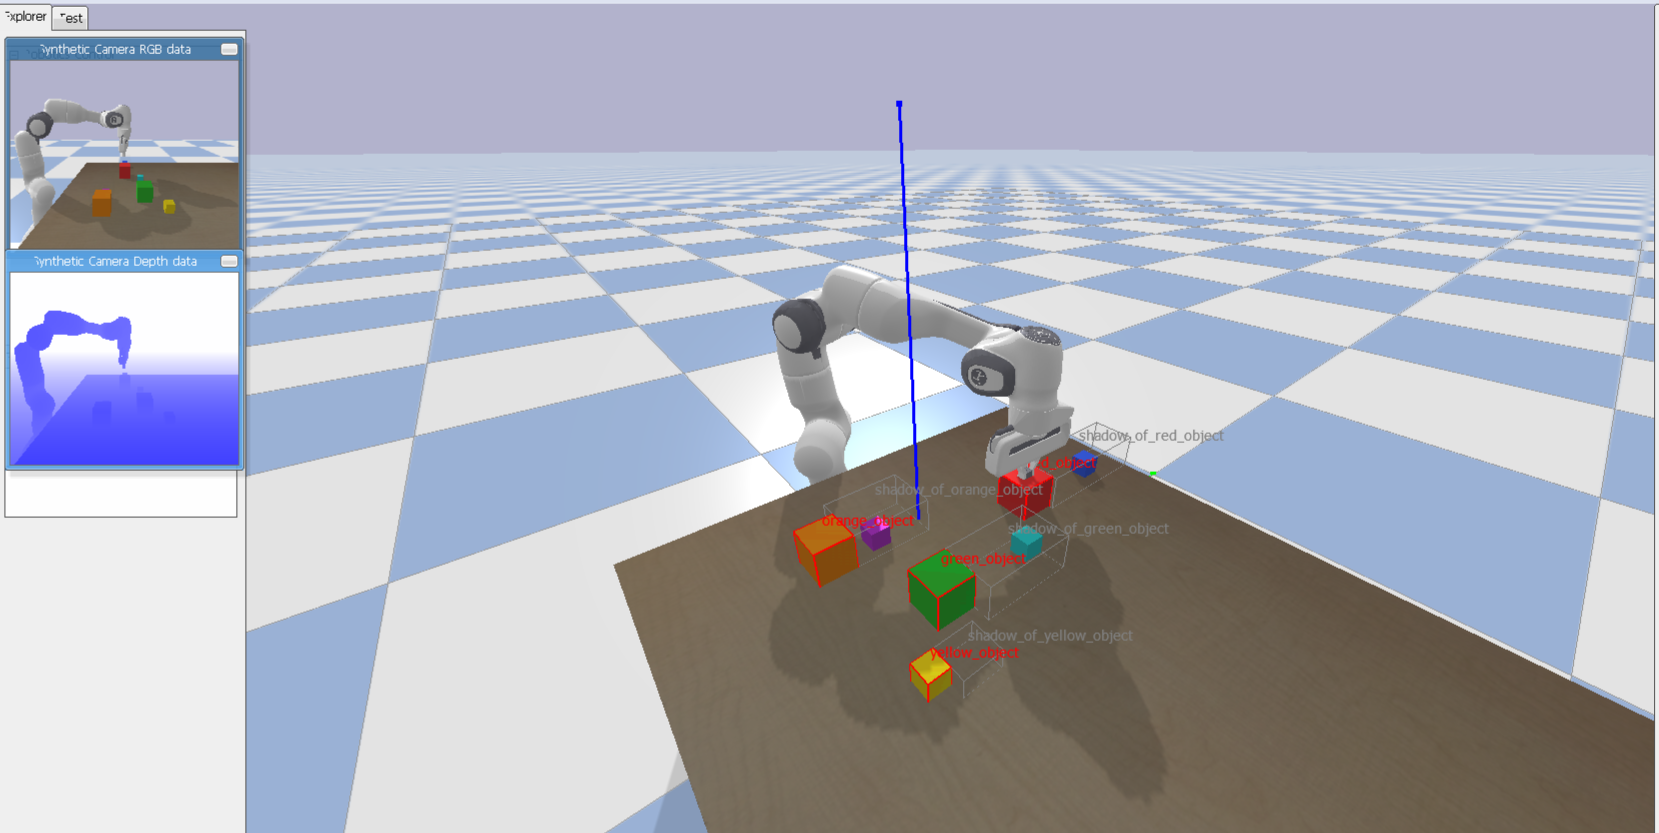
\includegraphics[width=0.85\textwidth]{sim/scene_hidden_target.png}
    \caption{A 7-DOF Franka Panda at a cluttered tabletop. The target, the cyan cube behind the green cube, is hidden from the overhead camera and must be located before it can be retrieved. The corner panels are the fixed overhead camera's synthetic RGB (top) and depth (bottom) views.}
    \label{fig:intro-hero}
\end{figure}

Addressing this limitation is the central focus of this thesis: extending PDDLStream to operate under partial observability. This includes the ability to represent and reason over belief states that capture uncertainty in continuous spatial variables. Naive representations, such as a uniform voxel grid over 3D space, make the belief space blow up in size and quickly become impractical to plan with. A useful belief representation must therefore be detailed enough to be expressive, yet small enough to plan with quickly.
The core research question is:
\textit{How can we formally define and integrate a belief representation based on semantic partitioning into a POD-TAMP framework?}
The stance of this thesis is simple: \emph{space is part of the planning problem}. Where a hidden object might be, and what blocks the view of it, are not details to be collapsed into a probabilistic occupancy grid but structure the planner should weigh directly. Here, we present a novel approach to discretizing the workspace around the objects the robot detects, the regions they occlude, and the free space between them. The unit of this discretization is the Semantic Boxel: a task-relevant, occlusion-aware axis-aligned box, built from objects' known 3D models, that the robot uses to represent its belief. Unlike a dense, uniform discretization, this provides a structured, scalable way to represent and reason about spatial uncertainty.

This thesis develops a system\footnote{Source code: \url{https://git.rwth-aachen.de/hani.alassiri.alhabboub/Semantic_Space_Abstractions}.} in which a robot, facing uncertainty about object locations, can plan and execute a sequence of information-gathering and manipulation actions. It reasons over abstract beliefs about which Boxels objects might occupy, using PDDLStream to connect this reasoning to continuous motion and manipulation. Sensing is a symbolic action evaluated against a fixed overhead camera, not a viewpoint the robot moves to; and because the underlying planner is classical, partial observability is handled by optimistic sensing with reactive replanning rather than contingent planning: each sensing action is assumed to yield the outcome the plan expects, and the system replans if execution shows otherwise. The result is a framework that makes planning under spatial uncertainty simpler and more reliable. The approach is demonstrated on tabletop hidden-object retrieval and stacking; the partial-observability mechanism is the contribution, and longer task horizons are a natural extension.

\section{Contributions of This Thesis}
The central contribution is a \emph{representation}: each volume the robot cannot see becomes a named region that a classical, \ac{pod} planner reasons over and resolves by sensing. The three components below deliver this representation; the evaluation correspondingly isolates it by ablation (the same planner on the adaptive partition against a uniform grid), rather than claiming a benchmark win, and is conducted under oracle perception (\cref{sec:limitations}).
\begin{itemize}
    \item The \emph{Semantic Boxel} abstraction: an occlusion-aware, object-centric partitioning of the workspace that concentrates resolution on the task-relevant regions (the objects themselves and the volumes they occlude) while covering the remaining free space with a few coarse cells, rather than partitioning all space uniformly.
    \item A Semantic POD-TAMP model that uses Know-If Fluents over Boxels (atoms marking whether the truth of a fact is known) as a compact belief representation, letting a classical PDDL planner reason about partial observability via optimistic sensing with reactive replanning.
    \item A PDDLStream realization of this model that combines the discrete Boxel belief with stream-certified continuous geometry, so that information-gathering and manipulation actions interleave within a single planning domain.
\end{itemize}

\section{Thesis Outline}
\Cref{ch:background} provides essential background on classical planning, reasoning under uncertainty, and the PDDLStream framework that this work builds upon. \Cref{ch:related-work} reviews related work in TAMP under partial observability, belief representation, and adjacent planning paradigms. \Cref{ch:methods} details the methodology, including the formalization of Boxels through adaptive semantic discretization, the Semantic POD-TAMP model, and the PDDLStream integration. \Cref{ch:results} presents the experimental setup, the metrics and baselines, and the headline evaluation results. \Cref{ch:discussion} interprets those results and consolidates the accepted simplifications. \Cref{ch:conclusion} summarizes the contributions and outlines directions for future work.

  % !TEX root = ../main.tex

\chapter{Background}
\label{ch:background}
This chapter builds up the pieces the thesis depends on, ending with PDDLStream and how 3D space is represented for planning.

\section{AI Planning Fundamentals}
\Ac{ai} planning produces a sequence of actions---a plan---that gets from a given initial state to a specified goal \cite{ghallab2004automated}.

\subsection{State-Space Models in Classical Planning}
Classical planning describes problems in a \textit{factored} representation: states are specified through the atoms that hold and actions through their effects on those atoms, rather than by enumerating every configuration of the world explicitly, which is infeasible for all but the smallest problems \cite{geffner2013concise, ghallab2004automated}.

A foundational language for this is \textbf{\acs{strips}} \cite{fikes1971strips}. A \textbf{state} is the set of ground atoms (propositions) true in a configuration of the world---for example, in a blocksworld with blocks A, B and a table, $\{\texttt{(on A B)}, \texttt{(ontable B)}, \texttt{(handempty)}\}$. An \textbf{action} $a$ is given by three sets of atoms: preconditions $\mathrm{pre}(a)$, an add-list $\mathrm{add}(a)$, and a delete-list $\mathrm{del}(a)$. Action $a$ is \textit{applicable} in a state $s$ iff $\mathrm{pre}(a) \subseteq s$, and applying it produces the successor state $(s \setminus \mathrm{del}(a)) \cup \mathrm{add}(a)$.

\textbf{\ac{pddl}} \cite{aeronautiques1998pddl} gives this a standardized, more expressive syntax, splitting a problem $P = \langle D, I \rangle$ into a domain $D$ and an instance $I$. The \textbf{domain} $D$ declares \textit{predicates} (relations such as \texttt{(on ?x ?y)}) and \textit{action schemas}---parameterized templates that generalize STRIPS operators, e.g.:
            \begin{lstlisting}[style=PDDL,  label=lst:pddl_stack_action]
                (:action stack
                    :parameters (?obj1 - block ?obj2 - block)
                    :precondition (and (holding ?obj1) (clear ?obj2))
                    :effect (and (on ?obj1 ?obj2) (not (holding ?obj1))
                                 (not (clear ?obj2)) (handempty) (clear ?obj1))
                )

            \end{lstlisting}
whose negative effects (\texttt{(holding ?obj1)}, \texttt{(clear ?obj2)}) form the delete-list and whose positive effects form the add-list. The \textbf{instance} $I$ lists the \textit{objects}, the \textit{initial state} $s_0$ (the ground atoms true at the start), and the \textit{goal} $g$ (ground atoms required in any goal state). Grounding the schemas---replacing their parameters by objects---yields the ground actions. PDDL also supports features beyond STRIPS, such as conditional effects (\texttt{(when <condition> <effect>)}), numeric fluents, and axioms (derived predicates).

This syntax induces a \textit{state model} $S(P) = \langle S, s_0, S_G, Act, A, f \rangle$ as its semantics \cite{geffner2013concise, hofmann2024learning}: $S$ is the set of all states; $s_0 \in S$ the initial state; $Act$ the set of ground actions; $A(s) = \{\, a \in Act : \mathrm{pre}(a) \subseteq s \,\}$ the actions applicable in $s$; $f(a, s) = (s \setminus \mathrm{del}(a)) \cup \mathrm{add}(a)$ the successor state for $a \in A(s)$; and $S_G = \{\, s \in S : g \subseteq s \,\}$ the goal states. A \textit{solution} (or \textit{plan}) is a sequence of actions $\sigma = [a_0, \dots, a_n]$ with $a_i \in A(s_i)$ and $s_{i+1} = f(a_i, s_i)$ that ends in a goal state $s_{n+1} \in S_G$; an \textit{optimal} plan minimizes length or an associated cost.
%Derived predicates allow the definition of new predicates whose truth values are logically inferred from the base predicates in the current state, rather than being directly changed by action effects. For example, one might define:
% \begin{lstlisting}[style=PDDL, language=Lisp, basicstyle=\ttfamily\scriptsize]
% (:derived (block_in_region ?b - block ?r - region)
%     (exists (?p - pose)
%         (and (at_pose ?b ?p)
%              (pose_in_region ?p ?r) ; Assuming pose_in_region is base or another derived
%         )
%     )
% )
% \end{lstlisting}
% This allows for more expressive and modular domain definitions.
\subsection{Classical Planning Algorithms and Fast Downward}
\label{subsec:planning-algorithms}
Given a compact \ac{pddl} encoding, a planner must search the state space it
implies for a path from $s_0$ to a goal state. Because that space grows
exponentially with the number of atoms, modern classical planners treat the
task as \emph{heuristic state-space search}: they expand states with an
informed search algorithm---greedy best-first search, or A\textsuperscript{*}
\cite{hart1968formal} when an optimal plan is required---guided by a heuristic
that estimates the remaining cost from each state to the goal
\cite{geffner2013concise}. The performance of such a planner depends almost
entirely on the quality of this heuristic.

What makes the approach \emph{domain-independent} is that these heuristics are
derived automatically from the PDDL description rather than supplied by hand.
The most influential family relaxes the task by ignoring delete-lists; because
solving even this relaxation optimally is hard, planners use tractable
approximations such as the max and additive heuristics and the FF heuristic,
which extracts a plan for the relaxed task and counts its actions
\cite{hoffmann2001ff, geffner2013concise}. A complementary family reasons over
\emph{landmarks}---facts that every valid plan must eventually make
true---and the LAMA planner combines landmark and relaxation heuristics in a
cost-based anytime search \cite{richter2010lama}.

\textbf{Fast Downward} \cite{helmert2006fast} is the classical planner used as
the search backend throughout this work; PDDLStream invokes it to solve each
symbolic planning problem once its streams have supplied the continuous values
that problem requires. Rather than operate on STRIPS propositions directly,
Fast Downward first translates the grounded task into a \emph{multi-valued}
representation (SAS\textsuperscript{+}), in which each variable takes exactly
one value from a mutually exclusive set instead of many independent Booleans.
From this encoding it builds a \emph{causal graph} that captures how the
variables depend on one another, and derives structure-aware heuristics (such
as the causal-graph heuristic) that guide a best-first search. This pairing of
an automatic multi-valued translation with structure-exploiting heuristics is
what lets Fast Downward scale to the grounded planning tasks that arise in
this work.

\section{Planning under Partial Observability}\label{sec:pod}
Classical planning's assumption of full observability is often violated in robotics. When an agent has incomplete information about the true state of the world, it must reason about its \textit{belief state}.

\subsection{Belief States, K-Literals, and Know-If Fluents}
A belief state represents the agent's current set of possible world states consistent with its history of actions and observations. We refer to the setting this thesis targets as \emph{Partially Observable Deterministic (POD)} planning: the world itself behaves deterministically and the only uncertainty is the agent's incomplete knowledge of the initial situation, which sensing resolves. POD builds on \cite{bonet2014flexible, albore2009translation, geffner2013concise}. The belief state $b$ is explicitly a set of possible states. Actions transition this set, and observations prune it.
A common way to reason about knowledge in POD planning is through K-literals \cite{bonet2011planning, geffner2013concise}. K-literals make the robot's knowledge about a proposition $p$ explicit. For example:
\begin{itemize}
    \item $K(p)$ signifies "$p$ is known to be true."
    \item $K(\neg p)$ signifies "$p$ is known to be false."
\end{itemize}
If neither $K(p)$ nor $K(\neg p)$ holds, the truth of $p$ is unknown. Separately, $p$ is "possibly true" whenever $K(\neg p)$ does not hold---which also covers the case where $p$ is known to be true.

K-literals are the basis of a \emph{translation} that compiles a partially observable problem into a classical one \cite{geffner2013concise}. Each literal $L$ of the original problem is replaced by the two fluents $K(L)$ and $K(\neg L)$~\cite{palacios2006compiling}; in the translated problem these are made true in the initial state only where the agent actually knows the corresponding value, and a literal whose value is unknown contributes neither. The translated problem therefore carries no uncertainty in its initial state and can be solved by an ordinary classical planner, which now searches for a plan that reaches a desired \emph{state of knowledge}---for example $K(\text{holding}(\text{target\_obj}))$, i.e.\ the agent knows it holds the target---rather than a desired world state. This thesis instead carries belief with \acp{kif}, the know-whether construct of Brenner and Nebel~\cite{brenner2009continual}. A Know-If fluent is weaker than a K-literal: rather than asserting that a fact is known true ($K(L)$) or known false ($K(\neg L)$), it records only that the agent knows \emph{whether} the fact holds---that its value is settled---while the value itself is carried by an ordinary fluent. The two are therefore not interchangeable: $K(L)$ commits to $L$ being true, whereas a \ac{kif} states only that $L$'s value is known and leaves that value to the underlying fact. We adopt \acp{kif} because the domain already stores where each object is, so it suffices to add one Know-If fluent per fact---whether that location is known---rather than two separate knowledge literals $K(L)$ and $K(\neg L)$ (\cref{sec:kif_belief}).

\subsection{Probabilistic vs. Deterministic Partial Observability}
POD planning differs from planning with \acp{pomdp} \cite{kaelbling1998planning}---a distinction that matters because we later compare our approach to POMDP-based TAMP. In POMDPs, the world is modeled as a \ac{mdp} with probabilistic transitions and observations, and the belief state is a probability distribution over world states. While highly expressive, POMDPs are computationally very demanding. POD planning assumes outcomes and observations are deterministic but unknown. This makes it more tractable than POMDPs, and it fits robotic problems where the uncertainty comes from not knowing the world rather than from actions behaving randomly.


\section{Task and Motion Planning (TAMP)}
\Ac{tamp} connects high-level task goals with a robot's actual physical movements \cite{garrett2021integrated}. The core problem is ensuring that a plan is physically possible. High-level planners often ignore geometry, leading to plans that seem correct but cannot be executed. Yet, including all geometric details from the start makes the problem too complex to solve. Combining high-level logic with real-world geometry is the central difficulty of TAMP, and frameworks like PDDLStream exist to bridge it.


\subsection{PDDLStream for TAMP}
PDDLStream \cite{garrett2018pddlstream} is a TAMP framework built to bridge this symbolic-continuous gap. It extends classical \ac{pddl} by introducing the core concept of \textbf{streams}.

\paragraph{Streams: declarative procedures for continuous parameters.}
A stream in PDDLStream is a procedure that generates or tests values for continuous parameters required by symbolic actions. These parameters might include object poses, robot configurations, grasp transformations, or motion trajectories. Streams have both a procedural and a declarative component:
\begin{itemize}
    \item \textbf{Procedural Component (Conditional Generator):} This is the actual code (e.g., a Python function) that, given some input values (which can be discrete symbols or other continuous values), produces a (potentially infinite) sequence of output values. For example, an \ac{ik} stream, given an object, its target pose, and a grasp, would generate a sequence of robot configurations that achieve that end-effector pose. A collision-checking stream, given a trajectory, would test if it is collision-free.
    \item \textbf{Declarative Component (Stream Specification):} This part is described in a PDDL-like syntax and informs  the symbolic planner what the stream does, what inputs it requires, what outputs it produces, and, crucially, what logical conditions (fluents) are associated with these inputs and outputs. This specification includes:
        \begin{itemize}
            \item \texttt{:inputs}: The typed parameters the stream procedure takes.
            \item \texttt{:domain}: A set of PDDL facts (preconditions) that must be true for the stream to be applicable for a given set of inputs. For example, an IK stream might require that a valid pose and grasp for the object are already known.
            \item \texttt{:outputs}: The typed parameters that the stream procedure generates.
            \item \texttt{:certified}: A set of PDDL facts that are guaranteed to be true if the stream successfully produces a set of outputs for given inputs. These "certified fluents" are added to the planner's state and represent new knowledge derived from the continuous domain. For instance, if an IK stream successfully finds a configuration \texttt{?q} for picking object \texttt{?obj} at pose \texttt{?p} with grasp \texttt{?g}, it might certify the fluent \texttt{(KinSolution ?obj ?p ?g ?q)}.
        \end{itemize}
\end{itemize}
PDDLStream employs a \textbf{lazy evaluation} strategy. Streams are not called exhaustively beforehand; instead, the symbolic planner calls them "on-demand" when it encounters an action whose preconditions require a continuous parameter to be instantiated or a continuous condition to be tested.

\paragraph{Example PDDLStream workflow.}
Consider a symbolic action \texttt{(pick ?obj ?p ?g ?q ?t)} (pick object \texttt{?obj} from pose \texttt{?p} using grasp \texttt{?g} via configuration \texttt{?q} along trajectory \texttt{?t}). For this action to be applicable:
\begin{enumerate}
    \item A stream might first be called to sample a stable \texttt{?p} for \texttt{?obj} on a surface. If successful, it certifies \texttt{(AtPose ?obj ?p)}.
    \item Then, another stream samples a grasp \texttt{?g} for \texttt{?obj}. If successful, it certifies \texttt{(Grasp ?obj ?g)}.
    \item An IK stream then takes \texttt{?obj, ?p, ?g} as input and tries to find a robot configuration \texttt{?q}. If successful, it certifies \texttt{(KinSolution ?obj ?p ?g ?q)}.
    \item Finally, a motion planning stream takes the current configuration and \texttt{?q} as input to find a collision-free trajectory \texttt{?t}, certifying \texttt{(Motion ?q\_start ?t ?q)}.
\end{enumerate}
Only if all these streams succeed and certify their respective fluents will the preconditions of the symbolic \texttt{(pick ...)} action be met.

The overall PDDLStream algorithm often reduces a TAMP problem to a sequence of finite PDDL problems, iteratively calling streams to discover more certified fluents until a complete, grounded plan is found. The original PDDLStream framework, however, was primarily designed for fully observable and deterministic settings.

\section{Spatial Representation for Robotic Planning}
\label{sec:spatial_representation}

A robot needs some way to represent the 3D space around it and the objects in it. Representing space is harder under partial observability, because the robot must also represent what it does not yet know.

\subsection{Discretization of Continuous Space}
Robots operate in continuous space, but symbolic planners reason over discrete states --- so the continuous space has to be discretized somehow.

\paragraph{Voxel grids.}
A common approach to represent 3D environments is to discretize them into a grid of uniform volumetric pixels, or \textbf{voxels}. Each voxel can store information, such as whether it is occupied, free, or unknown. While straightforward, uniform voxel grids can be memory-intensive and computationally expensive for large environments or high resolutions.

\textbf{Octrees} (\cref{fig:octmap_illustration}) \cite{hornung2013octomap} offer a more efficient hierarchical data structure for representing 3D space. An octree is a tree data structure in which each internal (non-leaf) node has exactly eight children, while leaf nodes have none. It starts with a single large voxel encompassing the entire space of interest. If this voxel is not homogeneous (e.g., it contains both free and occupied space), it is recursively subdivided into eight smaller child voxels (octants).
\begin{figure}[H]
    \centering % Centers the image
    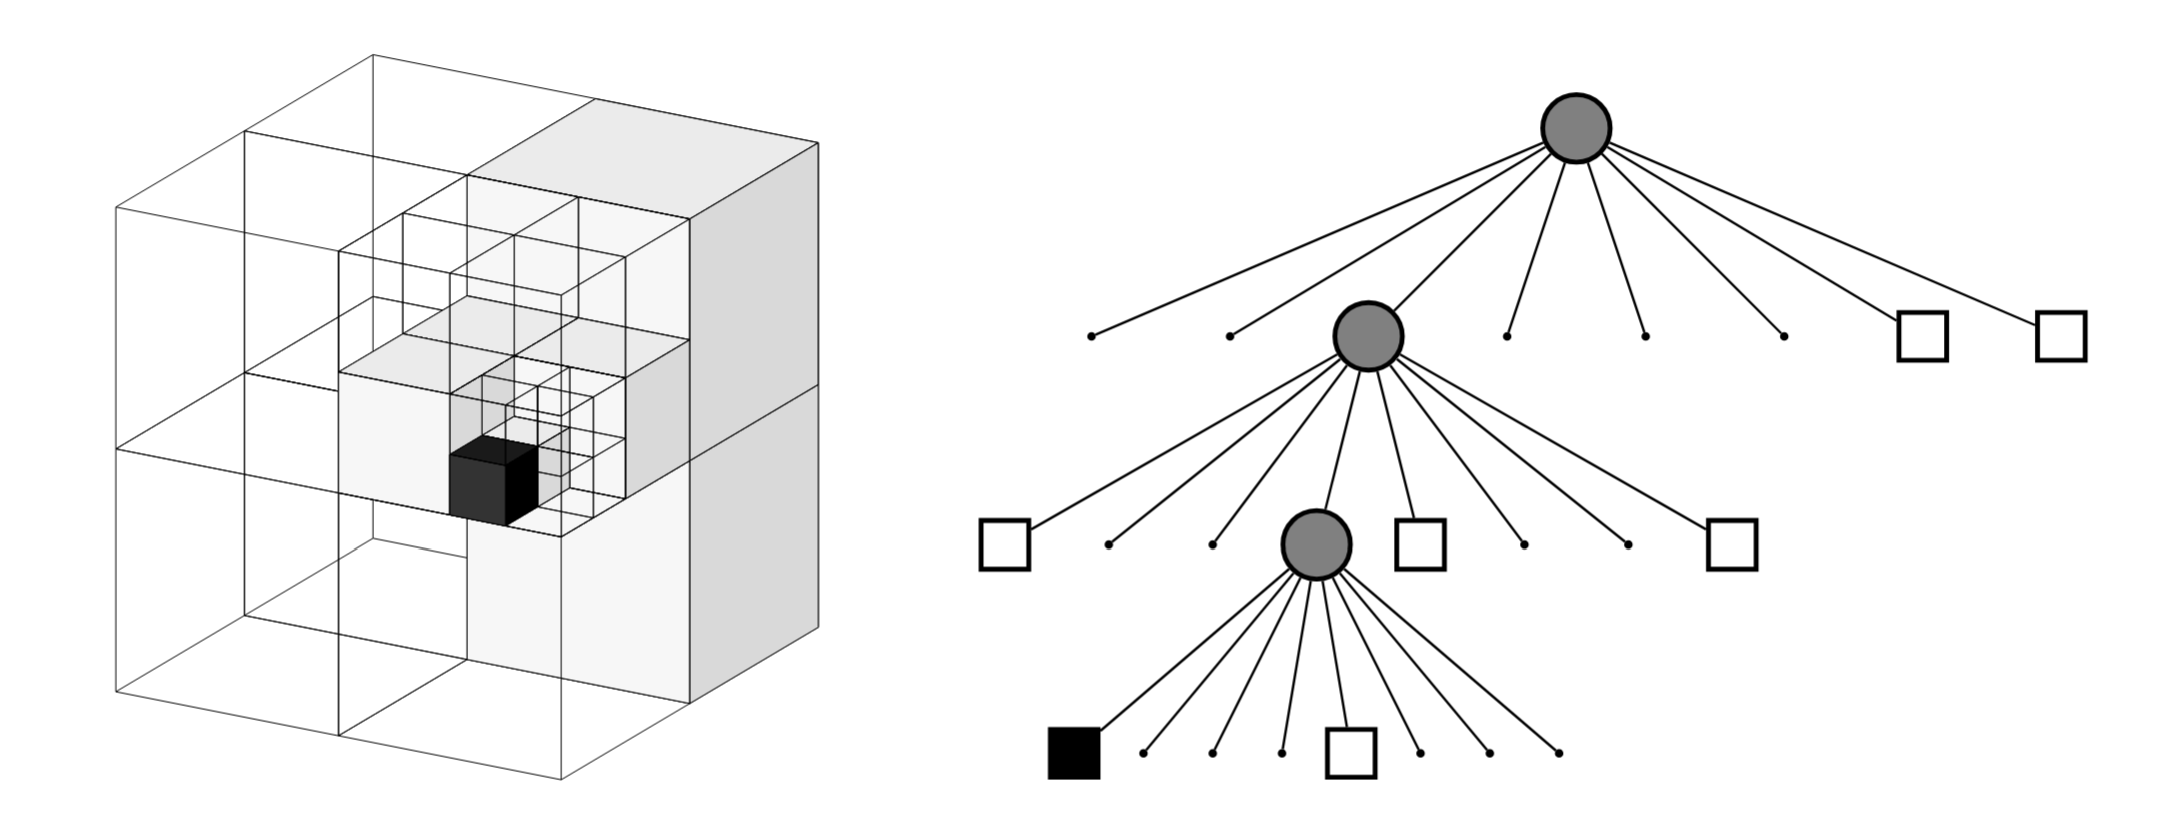
\includegraphics[width=0.65\textwidth]{octmap_illustration.png}
    \caption{Example of an octree storing free (shaded white) and occupied (black) cells. The volumetric model is shown on the left and the corresponding tree representation on the right.}
    \label{fig:octmap_illustration}
\end{figure}
This subdivision continues until voxels are homogeneous or a minimum resolution/maximum depth is reached. This process creates a tree where large, uniform regions (whether free, occupied, or unknown) are represented by single nodes at a shallower depth, making it highly efficient for representing sparse environments in comparison to uniform grid voxelization. The \textbf{OctoMap} framework \cite{hornung2013octomap} uses this principle to build probabilistic 3D occupancy maps from noisy sensor data. In such a framework, unobservable space is typically represented implicitly by the absence of nodes in a given volume; querying such a region returns an "unknown" status. The same octree structure also underpins learning-based 3D methods such as OctNet \cite{riegler2017octnet}, which runs deep convolutions efficiently on an octree rather than building an occupancy map; here it is the occupancy-mapping use that is relevant.

% Octrees are widely used in robotics for creating 3D occupancy maps from sensor data (e.g., OctoMap \cite{hornung2013octomap}), as they efficiently represent large free or unknown areas with fewer nodes.

% However, a limitation of standard Octree construction methods, when applied to planning under partial observability, is their typical reliance on direct sensor measurements (like point clouds) to guide subdivision based on observed point density or occupancy changes. This makes it challenging to use them directly to represent and reason about beliefs in unobserved or occluded regions where specific target objects might be hiding – a key focus for information-gathering plans.

\paragraph{Critical Regions.}
To make planning more efficient, space can be divided based on task-relevant meaning rather than uniform geometric criteria. One such approach is the concept of \textbf{\acp{cr}}, introduced by Molina et al.~\cite{molina2020learn} and later extended by Shah and Srivastava~\cite{shah2022abstractions}. In the original formulation, a critical region is a part of the configuration space with a low probability of being sampled by a uniform sampler yet essential to a solution---narrow passages such as doorways~\cite{molina2020learn}. Shah and Srivastava generalised this to regions where task-relevant features---controller success rates, object visibility, or transition likelihoods---change significantly~\cite{shah2022abstractions}.

In this line of work the regions are not hand-specified: a deep network is trained to \emph{predict} the critical regions of a given environment from that scene's input, and the predictor generalises to environments it was not trained on. Once predicted, a \ac{rbvd} partitions the configuration space around the CRs: each point is assigned to the nearest critical region, forming abstract states. Transitions between these abstract states define abstract actions, forming the backbone for hierarchical planning. By focusing computation on these task-relevant regions, this approach scales planning more effectively. In this formulation the regions are predicted once per environment and then held fixed, so they do not adapt as objects move within a scene during execution; later work in the same line learns abstractions that adapt as the task changes~\cite{nayyar2025option}, though for reinforcement learning rather than POD-TAMP.

Our work borrows the idea of task-relevant spatial regions, but constructs Boxels geometrically from detected objects and their occlusions rather than learning a region predictor (\cref{ch:methods}).

  % !TEX root = ../main.tex

\chapter{Related Work}
\label{ch:related-work}
Integrating task and motion planning with partial observability is challenging, particularly when a robot must act on incomplete information about its environment. This chapter reviews previous work along the two axes the thesis combines: spatial representations a planner can reason over (\cref{sec:rw-spatial}), the axis on which this thesis contributes, and planning approaches for TAMP under partial observability (\cref{sec:rw-potamp}).

\section{Spatial Representations for Planning under Occlusion}
\label{sec:rw-spatial}

The contribution of this thesis is a spatial representation, so the closest related work is not only other planners but other ways of carving up space. The standard choices, uniform voxel grids and octree occupancy maps such as OctoMap \cite{hornung2013octomap}, answer where matter is: each cell is occupied, free, or unknown, and unobserved space is represented implicitly, by the absence of evidence (\cref{sec:spatial_representation}). Nothing in the structure names which unknown volume matters to the task, which object hides it, or what must move for it to become visible; a planner searching for a hidden object would have to recover that meaning from raw geometry. Our evaluation keeps this family as the controlled baseline: the \texttt{uniform} variant (\cref{sec:baselines}) is exactly such a grid at the same cell size as the adaptive partition, so the measured gap isolates the structure of the partition rather than its resolution.

A second line abstracts space by task relevance instead of occupancy: learned critical regions \cite{molina2020learn, shah2022abstractions} partition the configuration space around regions that matter to solutions, such as narrow passages, and plan hierarchically over the resulting abstract states (\cref{sec:spatial_representation}). The regions, however, are predicted once per environment and held fixed, and the abstraction carries no notion of occlusion, so it neither names the volume hidden behind an object nor adapts when that object is moved; later work in this line that does adapt targets reinforcement learning rather than TAMP \cite{nayyar2025option}. Boxels keep the task-relevance idea but construct the regions geometrically, from the detected objects and their sightlines to the camera, and rebuild them whenever the scene changes.

Planning systems that do reason about occlusion represent it as a property of a probabilistic belief rather than as a region of space. TAMPURA's hidden-object benchmark keeps a visibility voxel grid that weights the success probability of its \texttt{look} action \cite{curtis2024partially}; IBSP carries maximum-likelihood occlusion fluents \cite{hadfield2015modular}; SS-Replan derives an occlusion predicate by ray-casting over its pose belief \cite{garrett2020online}; and occlusion-aware retrieval searches the likely poses of a hidden target under a learned distribution \cite{bejjani2021occlusion}. In each case occlusion is a check or a weight computed against a distribution over object poses, not a named occluded volume that a planner can sense, clear, or avoid re-blocking as symbolic state. That named-volume representation, constructed geometrically and held as deterministic planning state, is what the Boxel partition adds; \cref{sec:rw-potamp} reviews the planning frameworks it is evaluated against.

\section{TAMP under Partial Observability}
\label{sec:rw-potamp}
Existing approaches to TAMP under partial observability generally either use formal, probabilistic models or more ad-hoc, reactive methods, or a combination of both.

\subsection{POMDP-based TAMP Solutions}
Several works formulate planning under uncertainty as a POMDP to handle it in a principled, risk-aware way \cite{curtis2024partially, saleem2024pomdp}. \Ac{tampura} \cite{curtis2024partially}, for example, learns a coarse abstract model of each given controller's preconditions and effects, builds a non-deterministic MDP, and solves it with \ac{lao}, an uncertainty-aware solver \cite{hansen2001lao}, to produce risk-aware, information-gathering plans. \cite{saleem2024pomdp}, by contrast, addresses contact-rich \emph{manipulation} under object-pose uncertainty (not full task-and-motion planning), computing partial policies with an anytime heuristic-search POMDP solver.
However, a persistent challenge is the representation of belief over continuous properties, particularly object poses. TAMPURA \cite{curtis2024partially} samples object placements in continuous pose space and, in its real-robot pipeline, draws its object-pose belief from a perception front-end, Bayes3D \cite{gothoskar2023bayes3d}: a generative inverse-graphics model that infers a posterior over 3D scenes by rendering candidate object arrangements and scoring them against the observed depth image.

\subsection{Partially Grounded Plans in TAMP}
In contrast to formal probabilistic models, other TAMP systems handle uncertainty by deferring it to execution \cite{pan2024task}. These methods generate partially grounded plans, leaving ``gaps'' for actions with unknown outcomes. During execution, specialized closed-loop behaviors (hand-designed or learned) attempt to fill these gaps. If a controller fails, the failure is treated as a new constraint, and the system replans. This reactive approach avoids the need to model outcome probabilities explicitly. However, because it does not reason about uncertainty proactively, it can struggle with problems that require multi-step, strategic information gathering, such as deciding which of several actions is most likely to reveal a hidden object.

\subsection{Modern Approaches to TAMP under Uncertainty}
Recent works have leveraged learning and large models to address partial observability, offering different strategies than our own.

\cite{ma2025task} adds a strategic reasoning layer on top of a standard planner: it first reasons backward from an underspecified goal to decide which objects matter (Task-level Backward Search), then uses a constraint graph to order object moves collision-free through clutter (Object Manipulation Constraint Graph). We differ at the representation level rather than by adding a layer: we introduce a geometric belief representation, Boxels, so that the planner treats which regions are observed versus occluded as first-class planning state and information-gathering becomes a core planner action rather than a separate reasoning stage; the visibility signal is currently supplied by an oracle.

Another approach sources the planner's belief from large foundation models. \cite{zhao2025seeing} uses a \ac{vlm} as an uncertainty estimator: the VLM answers the planner's perceptual queries about an image (for example, ``Is the drawer empty?''), and the resulting belief feeds a \emph{symbolic} belief-space planner, a pairing of learned perception with structured reasoning that is reported to outperform end-to-end VLM planners. CoCo-TAMP~\cite{kim2026llmguided} is similar in spirit, drawing on the commonsense priors of a \ac{llm} to shape the belief over where task-relevant objects are likely to be, again within a partially observable TAMP loop. The difference from our work is the \emph{source} of the belief: theirs is learned (a VLM or LLM), whereas ours is a structured, object-centric geometric partition into discrete Boxels, with object poses currently supplied by a ground-truth oracle rather than a learned detector. Integrating a real detector is left to future work.

Finally, some methods move away from symbolic planning altogether and instead use end-to-end learning. \cite{bai2025learning} (TAVP), for example, uses a separate reinforcement-learning policy to select task-relevant \emph{virtual} camera viewpoints and re-render the scene from them, rather than physically moving the camera, and then produces the manipulation action with an end-to-end learned policy rather than a planner. This is fundamentally different from our model-based approach, where looking around is not a learned reflex but an explicit action chosen by the planner because its world model indicates that knowledge is missing. Because our method separates planning from execution, it is more transparent and can be retargeted to new goals without retraining a policy; the cost, however, is that a genuinely new goal requires authoring new PDDL actions and their streams, not just a new goal specification.

\subsection{Belief-Space Planning and Replanning}
A long line of work plans directly in \emph{belief space}, treating the robot's distribution over world states as the object of planning. \cite{kaelbling2013integrated} plans over the robot's belief using hierarchical goal regression, while \cite{hadfield2015modular} introduces a modular interface that exchanges information between an off-the-shelf classical planner and the geometric layer as the plan is built, determinising the problem under the maximum-likelihood-observation assumption so that a successful plan generates the observations it needs. A practical alternative to maintaining an explicit stochastic model is to \emph{determinise and replan}: SS-Replan \cite{garrett2020online} plans deterministically in a hybrid belief space and replans whenever a new observation arrives, including sensing actions within a single plan. Our system shares this determinise-and-replan strategy: we commit to an optimistic deterministic plan and replan on each observation rather than synthesising a probabilistic policy. What we add is separate from the replanning loop: a spatial belief in which occlusion is an explicit, named planning state, so information-gathering is explicitly composed within the planning representation.

\subsection{Partially Observable Deterministic Planning}
A separate tradition handles partial observability \emph{without} probabilities, by reasoning about what is \emph{known}. A prominent line within partially observable deterministic (POD) planning represents knowledge with explicit \emph{knowledge literals} (\cref{sec:pod}) and reduces the problem to classical planning by compilation; other POD planners instead search belief space directly, as in Contingent-FF~\cite{hoffmann2005contingent} and MBP~\cite{bertoli2001planning}. The translation-based contingent planner CLG \cite{albore2009translation} and the classical-replanning K-replanner \cite{bonet2011planning} established this reduction; LW1 \cite{bonet2014flexible} made it scalable with a \emph{linear} translation; and a parallel route compiles partial observability to \ac{fond} planning \cite{muise2014computing}. This thesis builds directly on the POD line: we carry Know-If Fluents (e.g.\ whether a region's contents are known) inside the PDDL state and let a classical planner reason over them.

To our knowledge, the deterministic, knowledge-literal POD line has not previously been combined with task and motion planning, nor used a geometric belief representation that makes \emph{which regions are occluded} part of the symbolic state. The systems that do reason about occlusion do so over probabilistic beliefs or learned models (\cref{sec:rw-spatial}), and partially observable TAMP systems increasingly source their belief from learned models \cite{zhao2025seeing, kim2026llmguided} or probabilistic abstractions \cite{curtis2024partially}; we are not aware of prior work that represents occluded volumes as named, object-centric symbolic state resolved by sensing within a PDDLStream TAMP loop, the gap this thesis addresses.

\section{Summary and Research Gap}
These approaches occupy distinct points in the design space. POMDP-based methods such as TAMPURA \cite{curtis2024partially} reason about uncertainty proactively but rely on a learned probabilistic transition model, and they keep the spatial belief sub-symbolic, so occluded regions are never a named, inspectable state that the planner can target. Reactive, partially-grounded methods \cite{pan2024task} avoid probabilistic modelling but cannot plan multi-step information-gathering. Belief-space replanning \cite{garrett2020online} determinises and replans, as we do, but does not make occlusion a first-class planning entity. The POD tradition \cite{bonet2014flexible} reasons about knowledge symbolically and deterministically, but has not been applied to TAMP or to spatial occlusion. We build on these lines: a POD task-and-motion planner whose spatial belief is an adaptive, object-centric partition (Boxels) in which occluded regions and their observed/occluded status are an explicit symbolic state. The planner thus reasons about \emph{where} information is missing and composes deliberate look-and-clear actions, without the cost and opacity of a learned probabilistic model. On the spatial side, \cref{sec:rw-spatial} positions the partition against the existing representations: occupancy structures carry no semantic notion of an occluded volume, learned task-relevance abstractions are predicted once per scene rather than reconstructed as objects move, and occlusion-aware planners keep occlusion inside a probabilistic belief. None names the occluded volumes that sensing must resolve, which is what the Boxel partition adds.

This position yields three advantages, each with a limitation we state plainly. (i) \emph{Occlusion is an inspectable state}: named observed-versus-occluded regions a reader can enumerate, rather than a sub-symbolic visibility grid feeding a learned outcome model~\cite{curtis2024partially}; the limitation is that the visibility signal is currently supplied by an oracle rather than a perception module. (ii) \emph{Uncertainty is handled without probabilities}: Know-If Fluents record what is known deterministically, with no per-action probability to estimate; the limitation is that the planner cannot rank actions by success likelihood and instead minimises plan cost and replans when an optimistic assumption fails. (iii) \emph{No MDP machinery is required}: a lightweight deterministic PDDL layer replaces the learned-MDP stack of POMDP-based TAMP~\cite{curtis2024partially}; the limitation is that optimistic determinise-and-replan is sound only while belief reflects observation.


  % !TEX root = ../main.tex

\chapter{Approach}
\label{ch:methods}

This chapter details the methodology for integrating a novel spatial abstraction, Boxels, into a Partially Observable Deterministic (POD) Task and Motion Planning (TAMP) framework built upon PDDLStream.
\section{Overview}
Our methodology links abstract belief representation to continuous geometric reasoning through three components:
\begin{enumerate}
    \item \textbf{Adaptive Semantic Discretization:} A dynamic procedure for partitioning the robot's workspace into a set of meaningful Semantic Boxels, i.e. semantically meaningful subspaces, based on detected objects and their known 3D models.
    \item \textbf{A Formal POD-TAMP Model:} A formal model that uses these Boxels as the foundation for its state representation, allowing a POD planner to reason about knowledge and uncertainty regarding object locations and unobstructed spaces.
    \item \textbf{PDDLStream Integration:} An implementation using custom PDDL fluents, actions, and streams that operate on the belief state over Boxels, realizing the formal model in PDDLStream.
\end{enumerate}

\section{Adaptive Semantic Discretization: Generating Boxels}
We build the Boxel abstraction through a process of \textit{adaptive semantic discretization}. This process dynamically generates a set of Semantic Boxels ($\mathcal{BX}_{\text{set}}$) by partitioning the workspace based on detected objects and the occlusions they create. It runs as a Python stage before each call to the planner---and is re-run between actions as the scene changes---rather than as a PDDLStream procedure. \Cref{fig:boxelization} illustrates the process.
\begin{figure}[H]
    \centering % Centers the image
    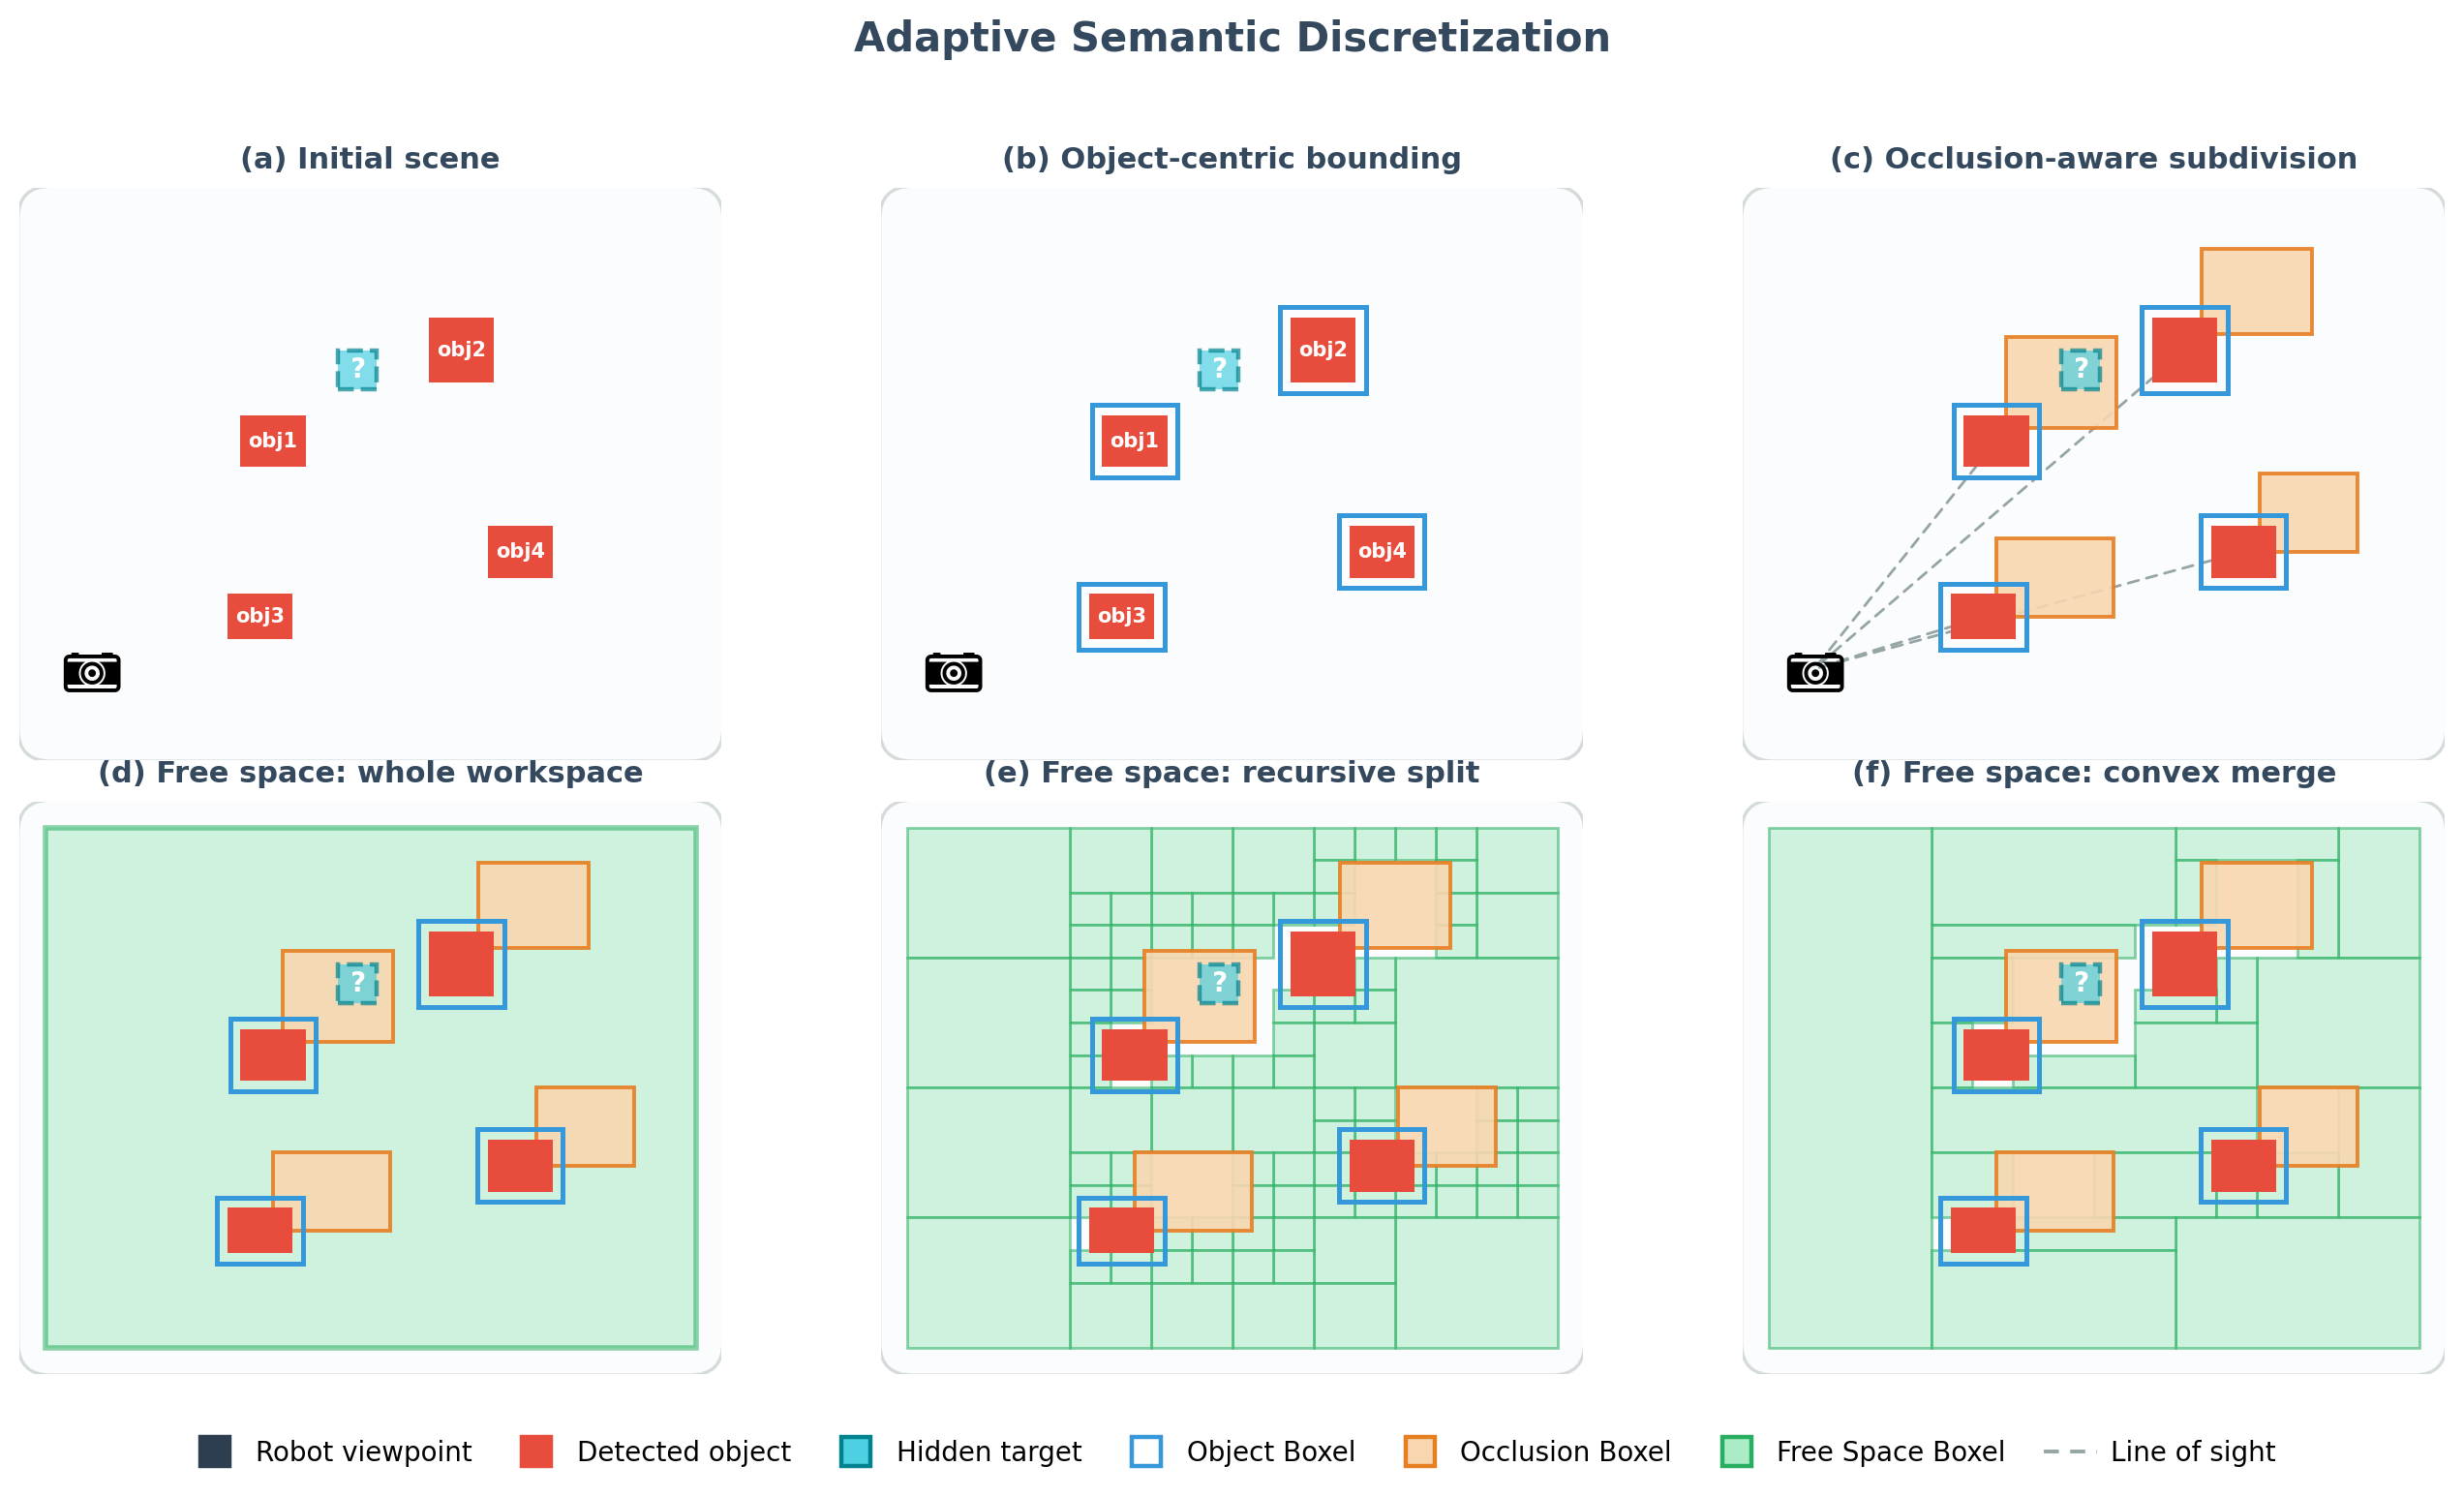
\includegraphics[width=\textwidth]{boxelization_stages.png}
    \caption{Adaptive Semantic Discretization Process. (a) Initial scene with robot viewpoint and detected objects. (b) Each object is bounded by a dedicated object Boxel. (c) The region each object occludes from the viewpoint becomes an occlusion (shadow) Boxel; dashed lines show the line of sight. (d)--(f) The remaining free space is partitioned: starting from a single cell spanning the whole workspace (d), cells overlapping any object or occlusion are recursively split (e), and the resulting free cells are greedily merged across aligned faces into larger convex Free Space Boxels (f).}
    \label{fig:boxelization}
\end{figure}

\begin{figure}[H]
    \centering
    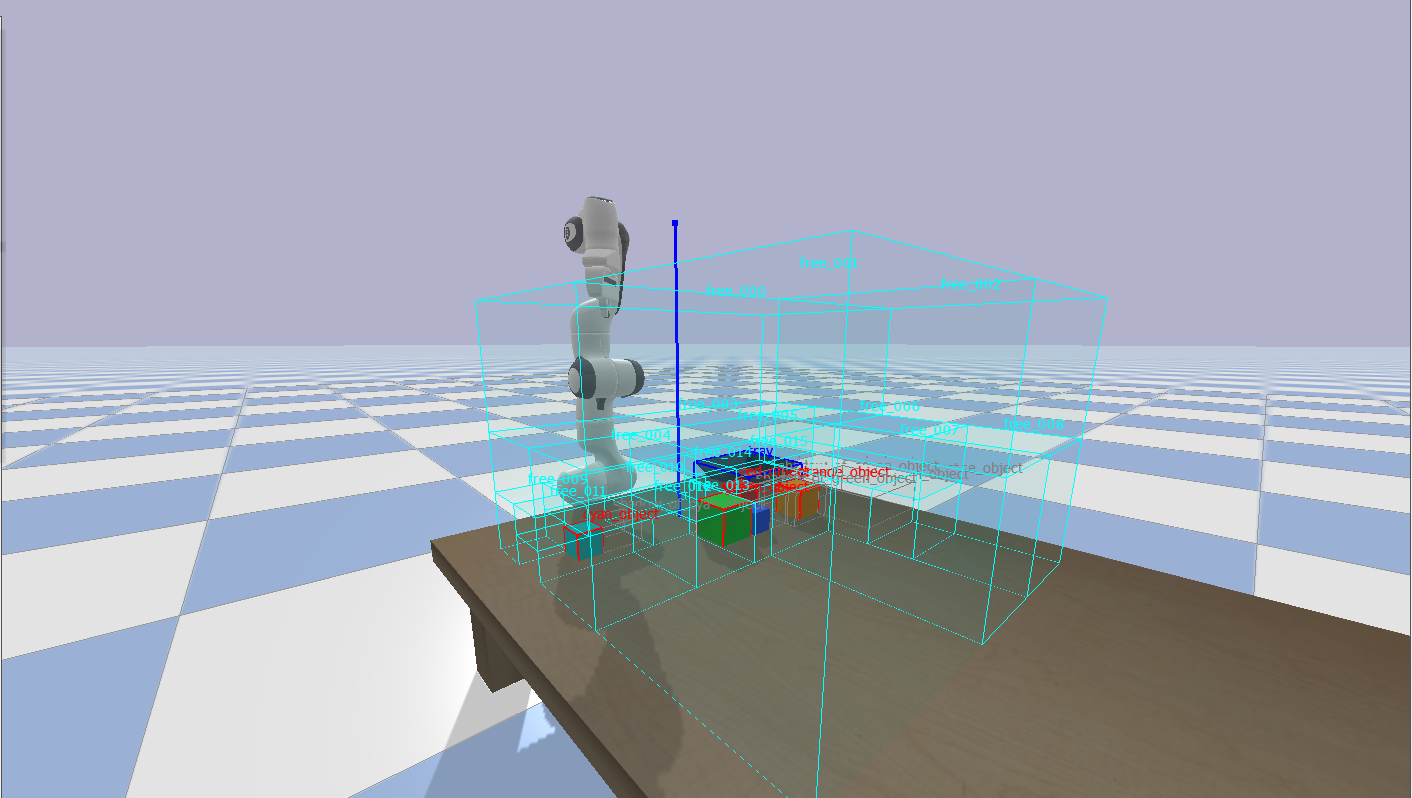
\includegraphics[width=0.8\textwidth]{sim/boxelization_real.png}
    \caption{The same partition applied to a PyBullet scene. The cyan wireframe cells are the Free Space Boxels filling the workspace; at the cube cluster, object bounding cuboids enclose the visible cubes and red wireframe Boxels mark the volumes they occlude.}
    \label{fig:boxelization-real}
\end{figure}

The generation process is as follows:
\begin{enumerate}
    \item \textbf{Object-Centric Bounding:} When an object is detected, we generate a dedicated Boxel: a cuboid that tightly bounds the object's known 3D model at its detected pose. This isolates each known object in its own spatial region. Object detection is provided by an oracle that returns ground-truth object identities and poses from the simulator, which isolates the planning contribution from perception noise; replacing it with a learned, image-based detector is left to future work.
    \item \textbf{Occlusion-Aware Subdivision:} For each object-bounding Boxel, the space occluded by it from the fixed camera viewpoint is calculated and partitioned into one or more shadow Boxels, split by any intervening visible obstacles. As the robot acts, the set of shadow Boxels is updated: sensing a region resolves its shadow, and discovering a previously hidden object adds a shadow for that object. A relocated object, however, is not given a new shadow at its destination. Re-creating shadows for moved objects could admit plans that never terminate, so it is deliberately omitted; handling it safely would require additional belief bookkeeping and is left to future work. This explicitly represents regions the robot currently cannot observe, so the planner can target them with information-gathering actions.

    \item \textbf{Recursive Partitioning:} The space not occupied by object or occlusion Boxels is partitioned recursively, starting from a single Boxel that spans the whole workspace. A Boxel found to be empty is kept as a Free Space Boxel; a Boxel that still overlaps an object or occlusion is split into eight octants, and the procedure repeats on each. Subdivision stops when a region is empty or a minimum Boxel size is reached. The resulting free cells are then merged greedily across shared faces into larger convex Boxels, which reduces their number without changing the represented free volume. This merge is convex-only---two cells are combined only when they share an exactly aligned face---so the partition retains more, smaller free Boxels than a full semantic merge would; this is accepted as sufficient for the object counts evaluated here (see \cref{sec:limitations}).
\end{enumerate}
This adaptive, object-centric approach contrasts with a uniform voxel grid by focusing discretization effort on task-relevant areas---the objects themselves and the occluded spaces they create---rather than partitioning all space uniformly. Its free-space stage is itself an octree, and a uniform-grid baseline is implemented for comparison. Each generated Boxel is assigned a unique ID and associated geometric data; the completed set of Boxels is supplied to the planner as static facts in its initial state. \Cref{fig:partition-comparison} contrasts the two partitions on a matching scene.

\begin{figure}[H]
    \centering
    \begin{subfigure}[t]{0.48\textwidth}
        \centering
        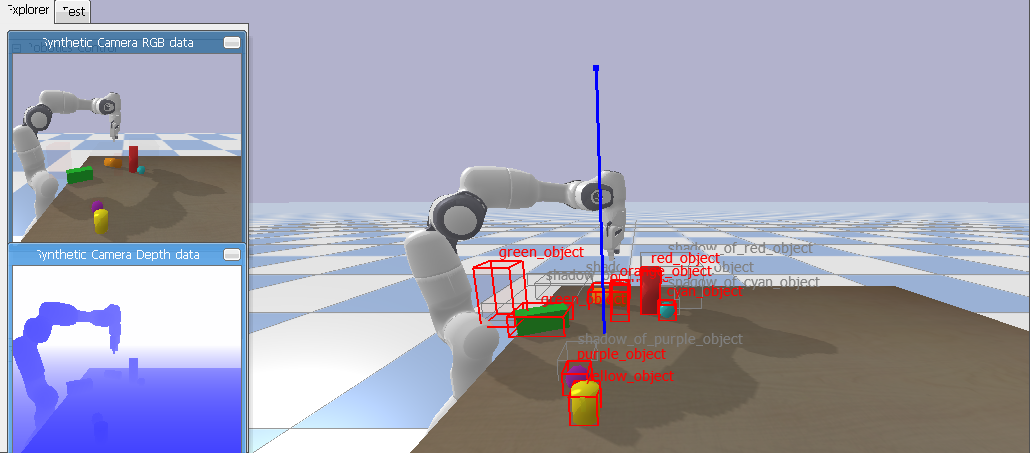
\includegraphics[width=\textwidth]{sim/partition_semantic.png}
        \caption{Semantic partition: cyan Free Space Boxels where the scene is empty, plus object and shadow Boxels at the cube cluster.}
        \label{fig:partition-semantic}
    \end{subfigure}
    \hfill
    \begin{subfigure}[t]{0.48\textwidth}
        \centering
        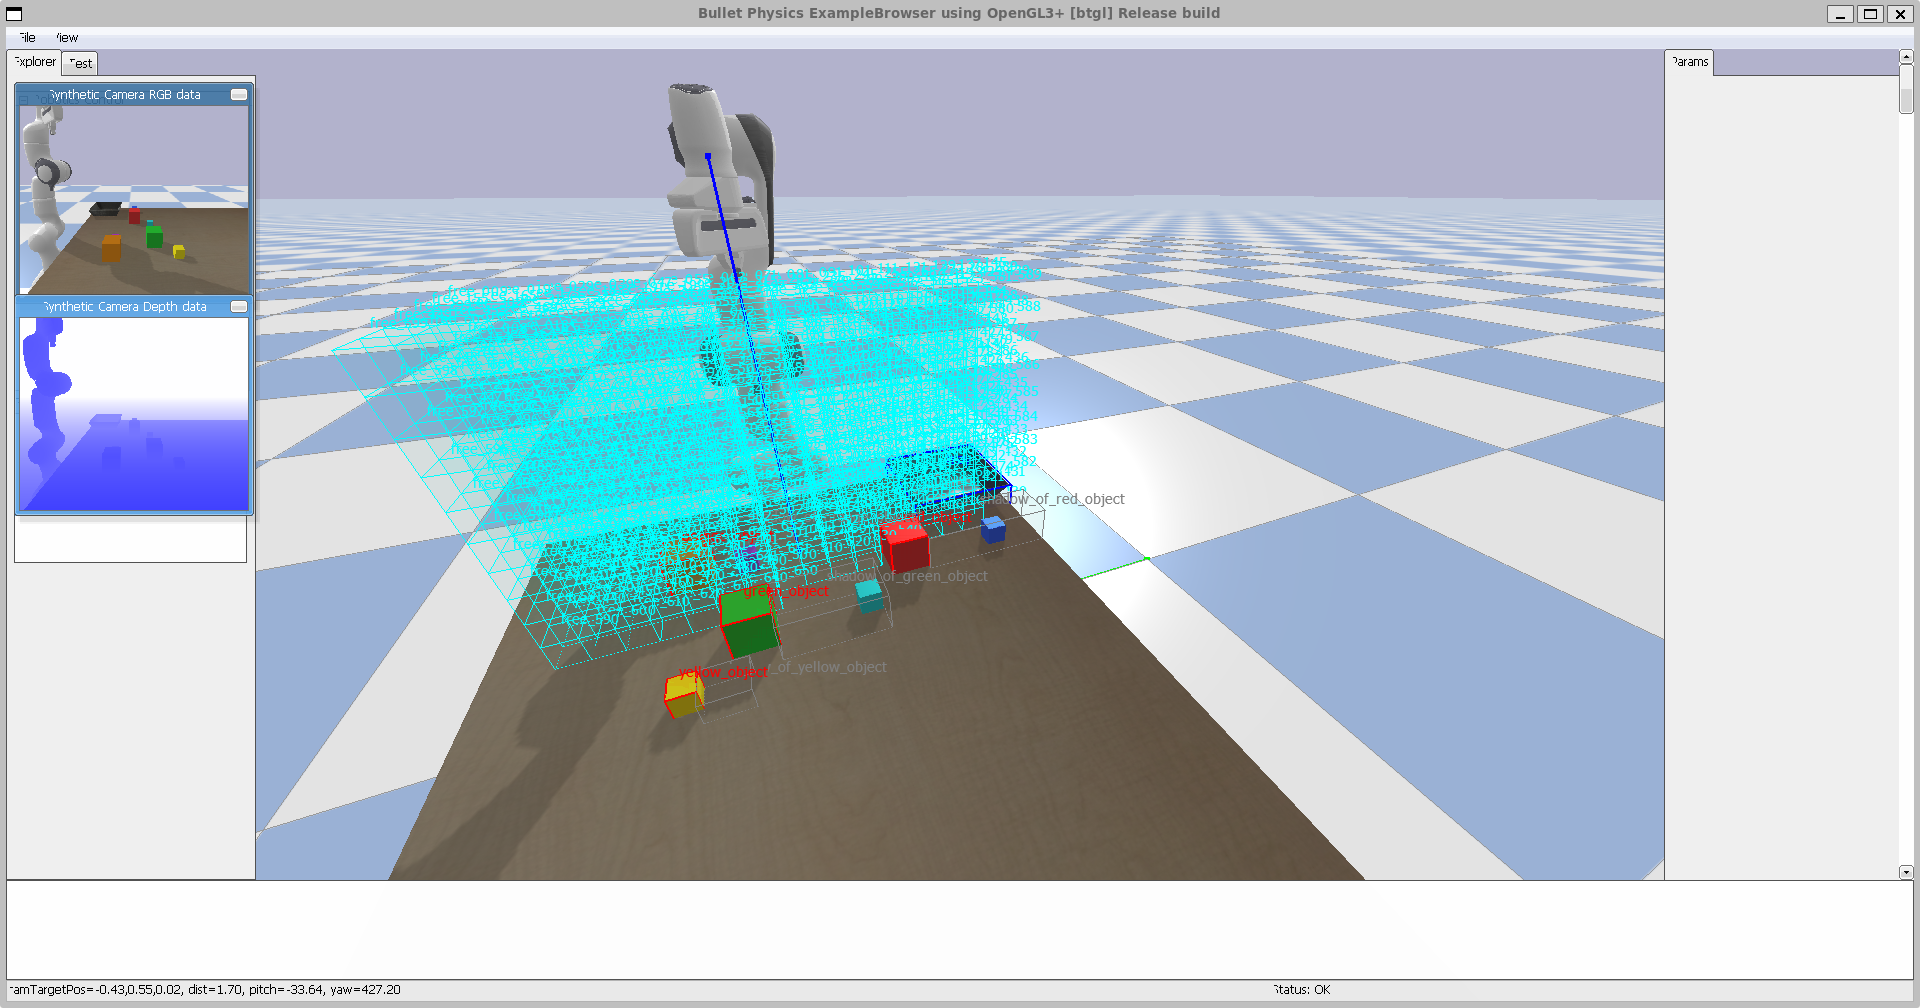
\includegraphics[width=\textwidth]{sim/partition_uniform.png}
        \caption{Uniform-grid baseline: hundreds of fixed-size cyan cells covering the whole workspace.}
        \label{fig:partition-uniform}
    \end{subfigure}
    \caption{Adaptive semantic partition (left) versus uniform-grid baseline (right) on a matching scene. The adaptive partition produces a small set of task-relevant cells; the uniform grid covers the whole workspace at the same cell size, producing an order of magnitude more cells.}
    \label{fig:partition-comparison}
\end{figure}

\section{Belief over Boxels with Know-If Fluents}
\label{sec:kif_belief}
The Semantic Boxels generated in the previous section partition the workspace into a finite set of regions; what the robot does not know is which Boxel a hidden object occupies. We represent this uncertainty with the Know-If Fluents introduced in \cref{ch:background}. For each object $obj$ and Boxel $Boxel$, the belief carries the K-literal $K(\operatorname{InBoxel}(obj, Boxel))$ when the robot knows the object is in that Boxel and $K(\neg \operatorname{InBoxel}(obj, Boxel))$ when it knows the object is not; the absence of both means the object is possibly there. Because the set of Boxels is finite, the belief over object locations is finite as well, and it is held directly in the planner's symbolic state.

Representing belief this way is what keeps planning tractable. As described in \cref{ch:background}, the K-literal translation compiles a partially observable problem into a classical one. Applied here, it lets an ordinary classical planner reason directly about where objects might be and plan sensing actions to resolve that uncertainty within the same classical search, rather than delegating belief to a separate contingent or belief-space planner. This compile-to-classical reduction is the one introduced by the POD planners CLG and LW1 \cite{albore2009translation, bonet2014flexible}; we adopt their knowledge-literal translation and solve the result by optimistic determinisation and reactive replanning (\cref{ch:related-work}): we assume each sensing action succeeds (optimistic), plan as if the world were fully known, execute, and replan whenever an observation contradicts that assumption (reactive replanning).

Knowing which Boxel holds an object is not enough on its own: a manipulation action also needs a reachable grasp and a collision-free trajectory. For this continuous-geometry side we rely on PDDLStream, which extends classical PDDL with \emph{streams}---the lazily-evaluated samplers and tests for continuous parameters described in \cref{ch:background}. Our approach combines the two in a single PDDL domain: Know-If Fluents carry the discrete belief over Boxels, while streams certify the continuous facts---grasps, inverse-kinematics solutions, and motions---that the manipulation actions require. A symbolic action such as picking a target object therefore mixes both kinds of precondition: a Know-If Fluent stating that the target's Boxel is known, and stream-certified geometric facts stating that the grasp and motion are feasible. The following two sections make this concrete, giving first the formal POD-TAMP model and then its PDDLStream realization.

\section{Semantic POD-TAMP Model Definition}
We formalize our Semantic POD-TAMP system as an explicit state model, adapting the state-space formulation of Geffner and Bonet~\cite{geffner2013concise} to the partially observable deterministic setting. The model is a tuple:
\[
\mathcal{M} = \langle \mathcal{S}, \mathcal{S}_0, \mathcal{S}_G, \mathcal{A}, f, \mathcal{O} \rangle
\]
where:
\begin{itemize}
    \item \textbf{$\mathcal{S}$ (States):} A finite set of abstract states. Each state is a consistent assignment of truth values to a set of atomic propositions $\mathcal{AP}$ built from K-literals (see \cref{ch:background}). These propositions are grounded in the Boxel representation, e.g., $K(\operatorname{InBoxel}(obj_k, Boxel_j))$.
    \item \textbf{$\mathcal{S}_0$ (Initial States):} The set of possible initial abstract states, representing the initial belief $b_0$.
    \item \textbf{$\mathcal{S}_G$ (Goal States):} The set of goal states to be reached with certainty, specified by a logical formula over $\mathcal{AP}$ (e.g., $K(\text{holding}(\text{target\_obj}))$).
    \item \textbf{$\mathcal{A}$ (Actions):} A set of abstract actions defined as PDDLStream action schemas that operate on the belief state, such as `sense` or `pick`.
    \item \textbf{$f$ (Transition Function):} A deterministic state-transition function $s' = f(a,s)$ that applies an action's add and delete effects to the current state, so that the successor state reflects the updated knowledge.
    \item \textbf{$\mathcal{O}$ (Sensor Model):} The sensor model relates a sensing action to the observation it yields---the target is found in a Boxel, or it is not---and the resulting belief update. In our system this is not realized as an observation function inside the POD planner: the planner's sensing action is optimistic and assumes the target is found, while the true outcome is obtained at execution time and folded into the belief by a Python sense-plan-act loop, which replans whenever the optimistic assumption proves wrong.
\end{itemize}
The planning problem is to find a sequence of actions from $\mathcal{A}$ that moves the belief state from $b_0 = \mathcal{S}_0$ to a belief state $b_g$ in which every possible state is a goal state (i.e., $b_g \subseteq \mathcal{S}_G$).

\section{PDDLStream Integration}
This section presents the implemented PDDL domain and streams that realize the model on the belief state over Boxels. For readability the listings show the belief-related fragment of the domain, eliding the geometric and stacking predicates that are not central to this discussion.

\subsection{PDDL Fluents for Belief Representation}
The agent's knowledge is represented directly in the PDDL state. The implemented domain is untyped STRIPS, so object categories are themselves predicates, and the belief over object locations is carried by a single Know-If fluent.
\begin{lstlisting}[style=PDDL, caption=PDDL fluents for belief over Boxels, label=lst:pddl_fluents_k_literal]
(:predicates
    ; --- Category predicates (untyped domain) ---
    (Boxel ?x)               ; ?x is a Boxel
    (Obj ?x)                 ; ?x is a manipulable object

    ; --- Boxel classification ---
    (is_shadow ?b)           ; ?b is an occluded region
    (is_object ?b)           ; ?b bounds a physical object
    (is_free_space ?b)       ; ?b is known-empty space

    ; --- Object location: value and knowledge ---
    (obj_at_boxel ?o ?b)     ; object ?o is at Boxel ?b
    (obj_at_boxel_KIF ?o ?b) ; Know-If fluent: it is known whether ?o is at ?b

    ; --- Other knowledge and robot state ---
    (obj_pose_known ?o)      ; ?o has been localized to a Boxel
    (handempty)              ; the gripper is empty
    (holding ?o)             ; the gripper holds ?o
    ; ... further robot, geometry, and stacking predicates
)
\end{lstlisting}
\Cref{sec:kif_belief} describes belief with the two K-literals $K(\operatorname{InBoxel})$ and $K(\neg\operatorname{InBoxel})$. The implemented domain realizes the same belief with a single Know-If fluent: \texttt{obj\_at\_boxel\_KIF} marks that the location of an object relative to a Boxel is \emph{known}, while \texttt{obj\_at\_boxel} carries the value; the absence of the Know-If fluent means the location is still uncertain. The two encodings are logically equivalent, and the single fluent keeps the grounded state smaller.

\subsection{The Sensing Action}
Information gathering is realized by a single \texttt{sense} action, which checks whether a target object is present in a given Boxel.

\begin{lstlisting}[style=PDDL, caption=The implemented sense action, label=lst:pddl_sense_k_literal]
(:action sense
    :parameters (?o ?region)
    :precondition (and
        (Obj ?o)
        (Boxel ?region)
        (view_clear ?region)                 ; line of sight to the region is clear
        (boxel_fits ?o ?region)              ; ?o physically fits inside ?region
        (not (obj_at_boxel_KIF ?o ?region))  ; only sense while the location is unknown
    )
    :effect (and
        (obj_at_boxel_KIF ?o ?region)        ; the location of ?o is now known
        (obj_at_boxel ?o ?region)            ; optimistic: assume the object is found here
        (obj_pose_known ?o)
        (increase (total-cost) 1)
    )
)
\end{lstlisting}
The action is \emph{optimistic}: its effect unconditionally asserts that the object is found in the sensed region. An earlier design used conditional effects that branched on a \texttt{found}/\texttt{not\_found} observation, which would let the planner build a multi-step search (``sense $A$; if empty, sense $B$'') within one plan. PDDLStream and its classical backend do not support such contingent planning, so the implemented domain commits to the optimistic outcome and relies on \emph{reactive replanning}: when execution reveals that the target is not in the sensed region, the execution loop updates the belief and replans. An empty region is recorded as clear; a region that instead turns out to hold a \emph{non-target} object has that object---and the new region it occludes---added to the partition, re-boxelizing the workspace before the next plan so the newly revealed occluder enters the belief rather than being discarded. With $N$ candidate regions this converges in at most $N$ replanning cycles and is functionally equivalent to a conditional plan executed in sequence. \Cref{fig:sense-action} shows the action targeting a shadow region in the simulator.

\begin{figure}[H]
    \centering
    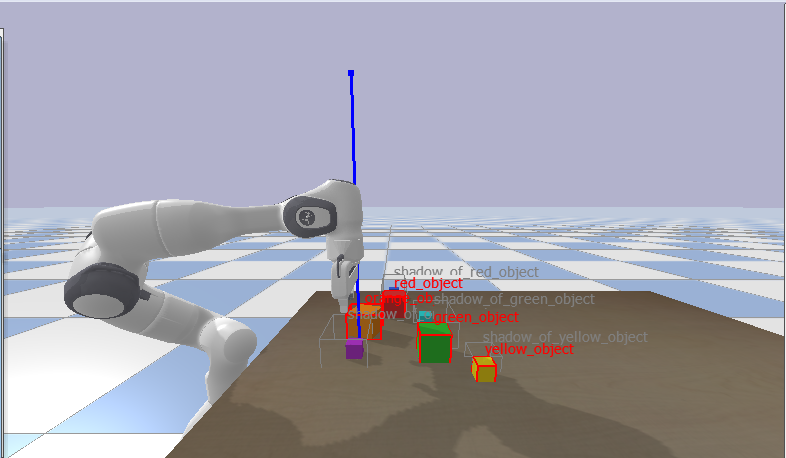
\includegraphics[width=0.85\textwidth]{sim/sense_targeting_shadow.png}
    \caption{The \texttt{sense} action targeting a shadow region in PyBullet. The arm has been moved to a sensing configuration over a labelled shadow; the in-simulator overlay labels each object and its shadow region. This is the configuration in which the \texttt{sense} action's \texttt{(view\_clear ?region)} precondition is checked and its optimistic \texttt{(obj\_at\_boxel ?o ?region)} effect is asserted.}
    \label{fig:sense-action}
\end{figure}

One bounded exception to this observation-driven belief update concerns regions that cannot be observed at all: if the line of sight to a shadow remains blocked after a fixed number of sensing attempts, that shadow is marked empty without ever being directly observed. This keeps the planner progressing when a region is effectively unreachable, but it is unsound---the region could still hold the target. A sound treatment, which would re-ground the view-blocking facts so the planner first clears the obstruction, is left to future work.

The sense action calls no streams. Because a fixed overhead camera observes the scene, no robot sensing configuration has to be sampled, and the only geometric precondition is the derived predicate \texttt{(view\_clear ?region)}, which holds when no object blocks the line of sight to the region. Streams instead serve the manipulation actions: the domain declares \texttt{sample-grasp}, \texttt{plan-motion}, \texttt{compute-kin}, and \texttt{compute-stack-kin}, so that an action such as \texttt{pick} requires a valid grasp, an inverse-kinematics solution, and a collision-free motion, each certified by a stream.

  % !TEX root = ../main.tex

\chapter{Evaluation}
\label{ch:results}

This chapter reports the experimental evaluation of the Boxel-based POD-TAMP framework. \Cref{sec:setup} describes the experimental setup as executed. \Cref{sec:metrics} defines the measured quantities. \Cref{sec:baselines} defines the variants compared, including the TAMPURA external reference. The results themselves follow in the remaining sections.

\section{Experimental Setup}
\label{sec:setup}

\paragraph{Simulator and robot.} All experiments were run inside PyBullet \cite{coumans2021pybullet}, with a 7-DOF Franka Emika Panda as the manipulator on a tabletop.

\paragraph{Goals.} Three goals were evaluated (\cref{fig:eval-tasks}):
\begin{itemize}
    \item \texttt{holding}: the robot must end the episode holding a single target object whose initial pose is hidden behind one of a set of occluders. The number of occluders $n_\text{occ}$ is the difficulty axis (2, 3, 4; see \cref{fig:n-occ-scale}).
    \item \texttt{stack}: the robot must build a stack of cubes to a given height. The stack height $h$ is the difficulty axis (2, 3, 4); cube positions are fully observable.
    \item \texttt{find-and-tray-stack}: the robot must locate hidden cubes behind occluders and stack them on a tray. The number of occluders $n_\text{occ}$ is the difficulty axis (2, 3, 4).
\end{itemize}

\begin{figure}[H]
    \centering
    \begin{subfigure}[t]{0.32\textwidth}
        \centering
        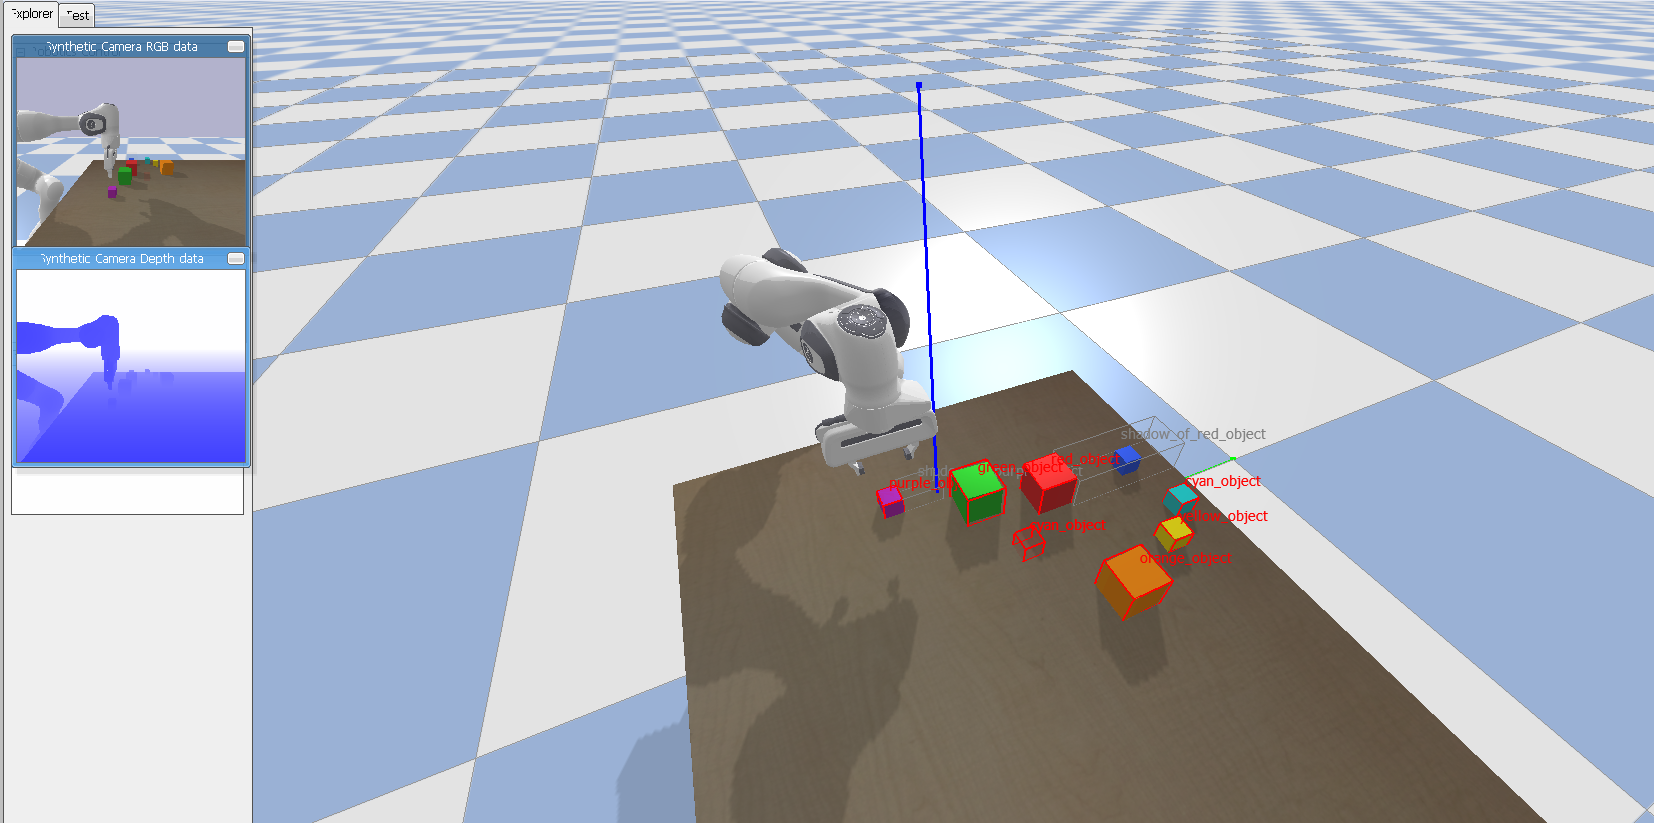
\includegraphics[width=\textwidth]{sim/task_holding.png}
        \caption{\texttt{holding}}
        \label{fig:task-holding}
    \end{subfigure}
    \hfill
    \begin{subfigure}[t]{0.32\textwidth}
        \centering
        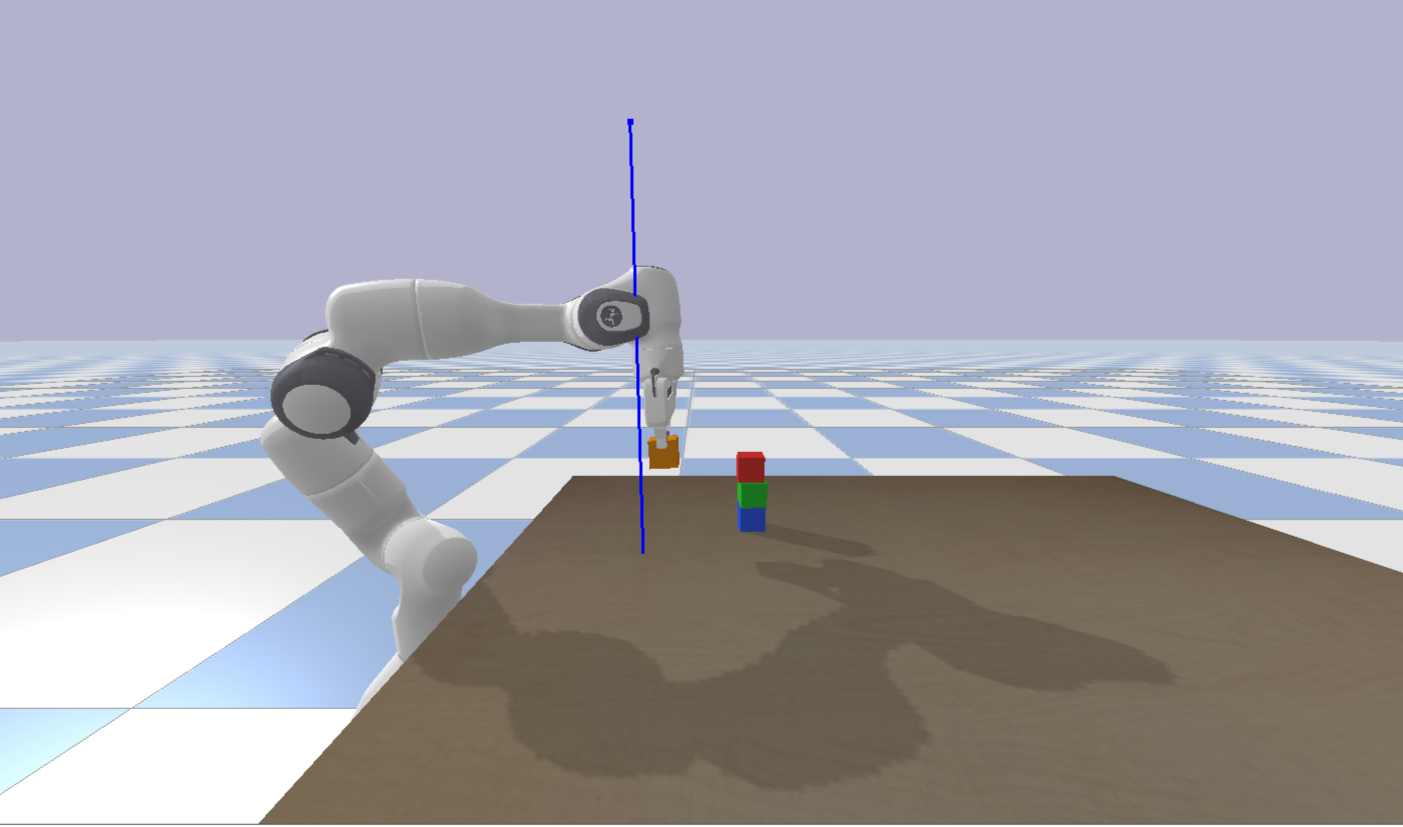
\includegraphics[width=\textwidth]{sim/task_stack.png}
        \caption{\texttt{stack}}
        \label{fig:task-stack}
    \end{subfigure}
    \hfill
    \begin{subfigure}[t]{0.32\textwidth}
        \centering
        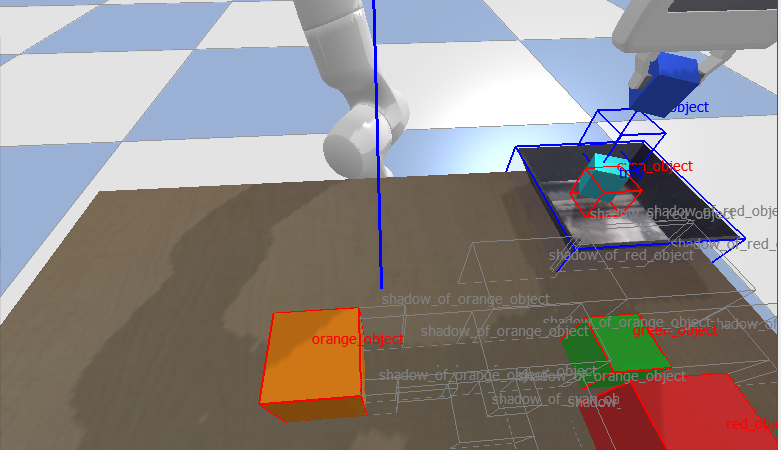
\includegraphics[width=\textwidth]{sim/task_tray.png}
        \caption{\texttt{find-and-tray-stack}}
        \label{fig:task-tray}
    \end{subfigure}
    \caption{The three evaluated goals. \texttt{holding}: retrieve a single target hidden behind occluders. \texttt{stack}: build a tower of cubes to a target height. \texttt{find-and-tray-stack}: locate hidden cubes and stack them on a tray.}
    \label{fig:eval-tasks}
\end{figure}

\begin{figure}[H]
    \centering
    \begin{subfigure}[t]{0.32\textwidth}
        \centering
        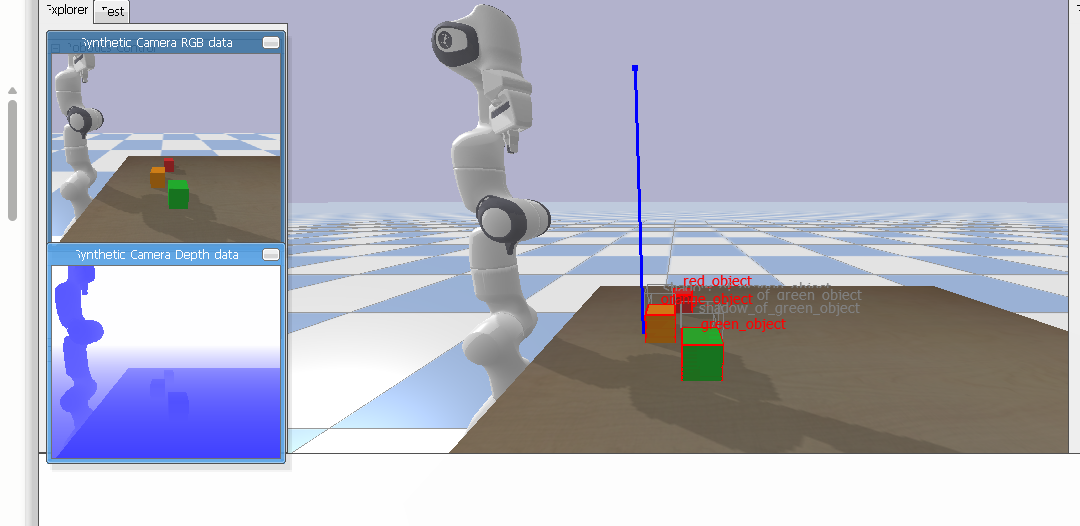
\includegraphics[width=\textwidth]{sim/n_occ_low_real.png}
        \caption{Low $n_\text{occ}$}
        \label{fig:n-occ-low}
    \end{subfigure}
    \hfill
    \begin{subfigure}[t]{0.32\textwidth}
        \centering
        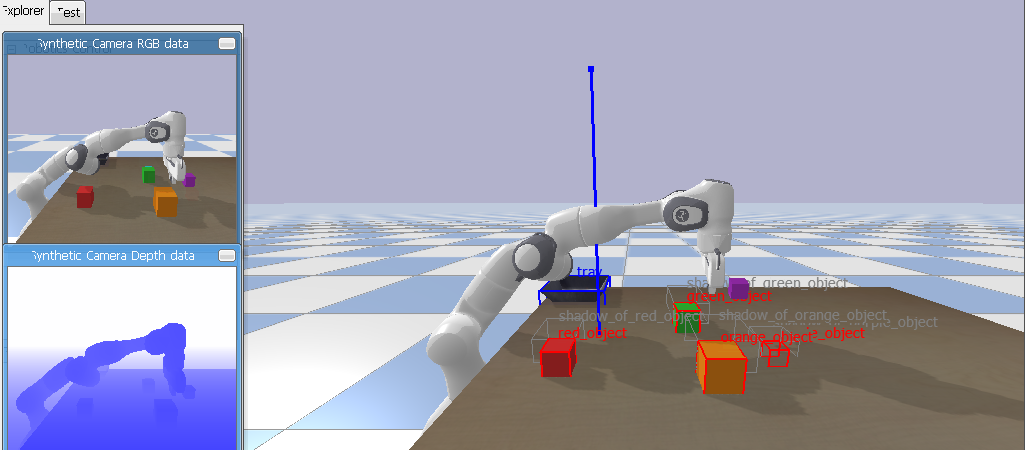
\includegraphics[width=\textwidth]{sim/n_occ_mid.png}
        \caption{Medium $n_\text{occ}$}
        \label{fig:n-occ-mid}
    \end{subfigure}
    \hfill
    \begin{subfigure}[t]{0.32\textwidth}
        \centering
        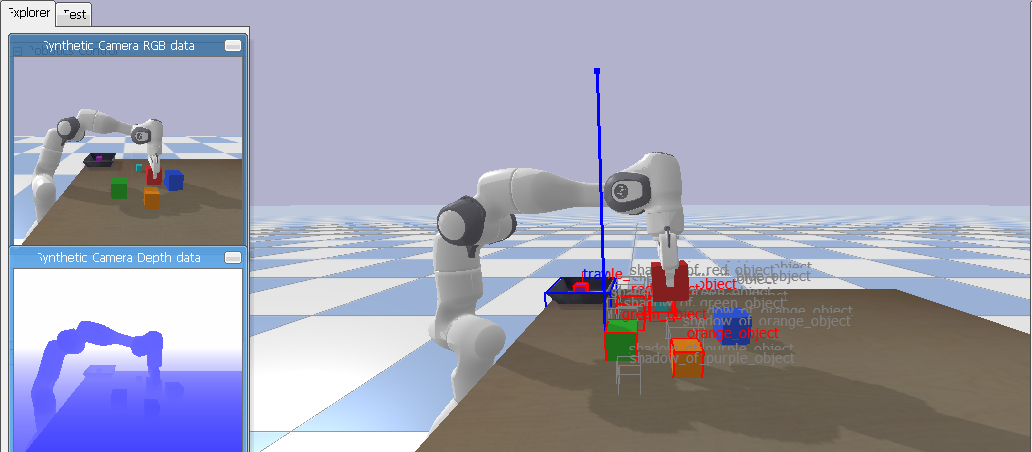
\includegraphics[width=\textwidth]{sim/n_occ_high.png}
        \caption{High $n_\text{occ}$}
        \label{fig:n-occ-high}
    \end{subfigure}
    \caption{The occluder-count difficulty axis $n_\text{occ}$, shown at low, medium, and high settings. More occluders crowd the target and occlude a larger share of the workspace, so the planner must reason over more shadow Boxels.}
    \label{fig:n-occ-scale}
\end{figure}

\paragraph{Scenes and seeds.} Each $(\text{goal}, \text{variant}, \text{difficulty})$ combination was run on 100 random scenes; seeds are paired across the \texttt{semantic} and \texttt{semantic+mbs0.05} variants on the random-pairs scene, so their head-to-head comparison is seed-for-seed. A total of $\approx$2700 cells were executed (3 goals $\times$ 3 variants $\times$ 3 difficulty levels $\times$ 100 seeds, with minor rounding from scheduling).

\paragraph{Perception.} Object detection is performed by an oracle that reads ground-truth object poses from the simulator and uses ray-casts from a fixed overhead camera (\cref{fig:overhead-camera}) to determine which objects, and which Boxels, are visible. The simulator also renders RGB-D images, but they are not processed inside the planning loop. The modelled uncertainty is occlusion uncertainty---which Boxel a hidden object occupies---resolved at run time by the \texttt{sense} action.

\begin{figure}[H]
    \centering
    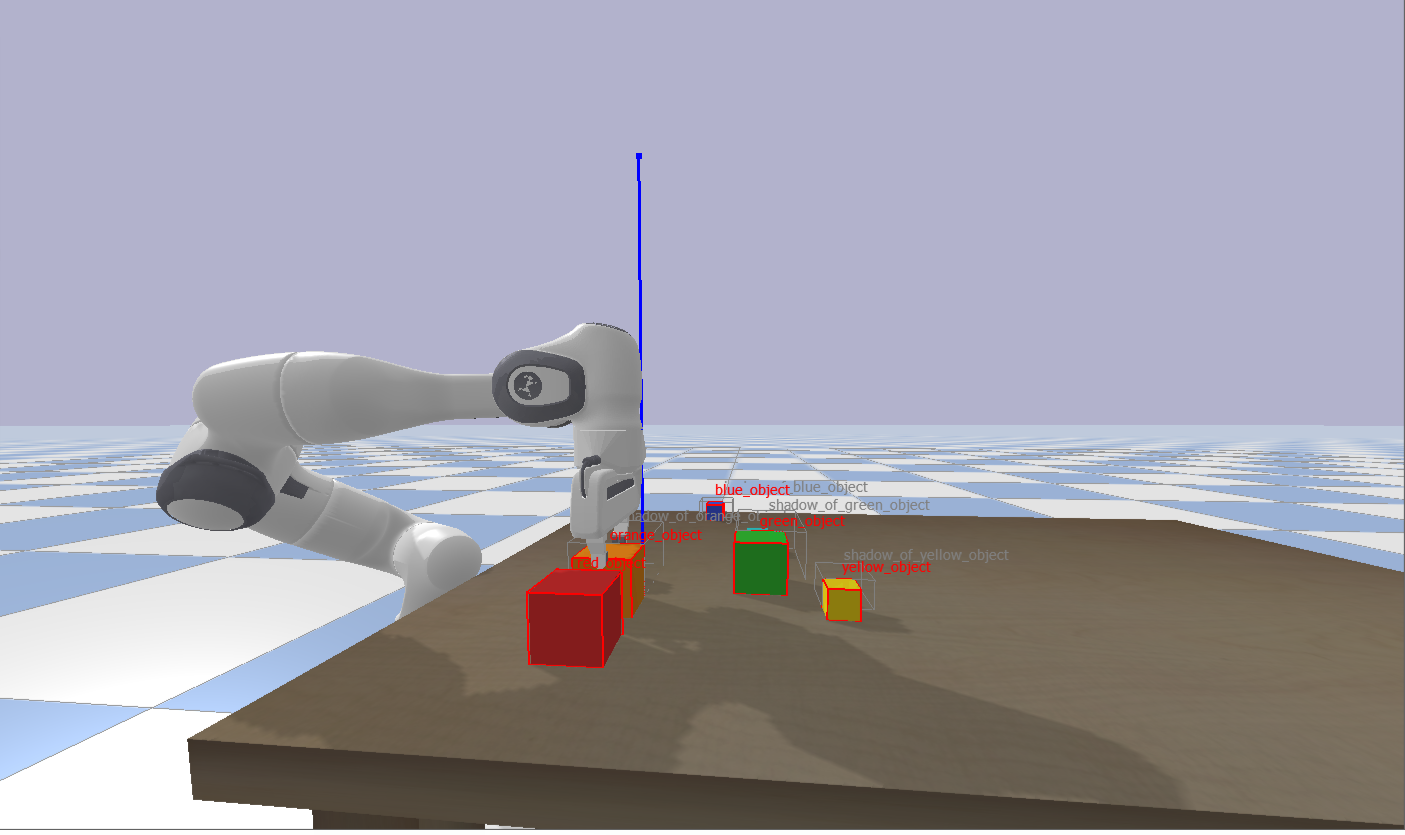
\includegraphics[width=0.85\textwidth]{sim/overhead_camera_inset.png}
    \caption{An evaluation scene observed by the fixed overhead camera, shown here from an oblique simulator viewpoint. Object detection is an oracle that reads ground-truth object poses from the simulator---objects and their occlusion shadows are labelled in the overlay---rather than processing the camera's rendered RGB-D images. A future learned detector would consume those images in place of the oracle, without changing the planning architecture.}
    \label{fig:overhead-camera}
\end{figure}

\paragraph{Planning budget.} Each PDDLStream call (initial plan or replan) was given a wall-clock budget of 1800\,s (30 min); a cell terminates with the \texttt{timeout} exit reason if it exhausts this budget. Most successful cells finish in well under a second per call; the budget exists to catch pathological cases rather than as the operating point. The anytime sweep records cumulative solve rate as a function of wall-clock budget, and the curves are essentially flat past $\approx$200\,s.

\paragraph{Software.} PyBullet \cite{coumans2021pybullet}; PDDLStream \cite{garrett2018pddlstream} with the FastDownward classical planner backend; Python 3.10.

\section{Evaluation Metrics}
\label{sec:metrics}

For each cell we record:
\begin{itemize}
    \item \textbf{Success}: whether the robot reached the goal within the planning budget, without exceeding the per-episode replan limit.
    \item \textbf{Planning time}: total wall-clock time spent inside PDDLStream calls, summed across replans. Wall-clock per cell is effectively equal to planning time; execution, perception, and motion overhead are negligible at the scales evaluated.
    \item \textbf{Replan count}: how many times the planner was re-invoked in the sense-plan-act loop before terminating.
    \item \textbf{Representation size}: the Boxel set decomposed into \texttt{OBJECT}, \texttt{SHADOW}, and \texttt{FREE\_SPACE} cells, and the number of grounded facts in PDDLStream's initial state. These two capture the per-cell cost of the partitioning strategy independently of planner choice.
    \item \textbf{Failure mode}: when a cell does not succeed, an exit reason among \texttt{planner\_failed}, \texttt{timeout}, \texttt{replan\_limit}, \texttt{physics\_mismatch}, \texttt{drop\_failed}, \texttt{no\_summary}, and \texttt{all\_searched}.
\end{itemize}
Aggregate means in this chapter are taken either over all $n_\text{cells}$ or, for quantities that are only defined on cells that produced a snapshot (notably mean initial-state facts and mean replan count), over the subset of cells with non-null values. The two denominators differ by $\sim$6\,\% of cells (early timeouts without a recorded state).

\section{Baselines for Comparison}
\label{sec:baselines}

Three variants of the planner are compared, plus one external reference:
\begin{enumerate}
    \item \textbf{semantic} --- the adaptive Boxel partition described in \cref{ch:methods}. Free-space cells are placed only where the workspace is empty; their leaf size is auto-set to the largest object's footprint ($\approx$6--9\,cm), since finer leaves break placement on the table dimensions used here.
    \item \textbf{semantic+mbs0.05} --- the same adaptive partition but with the free-space leaf-size floor forced to 5\,cm (\texttt{min\_boxel\_size = 0.05}). This is intended to test the effect of a finer free-space leaf floor independently of the semantic structure.
    \item \textbf{uniform} --- the adaptive partition is replaced by a uniform voxel grid over the workspace; the object and shadow Boxels are unchanged. The cell size is auto-set to the same largest-object-footprint value, since finer cells likewise break placement. This isolates the contribution of the adaptive free-space partition.
    \item \textbf{TAMPURA} \cite{curtis2024partially} --- a published POMDP-based TAMP framework. Its Table~II reports several model-learning/search configurations on a \textit{Partial Observability} task; we compare against TAMPURA's own primary configuration there---Bayes-Optimistic belief updates with LAO* search---which it reports at 57\,$\pm$\,38\,s over 20 trials (Table~II of \cite{curtis2024partially}, arXiv\,v2), rather than re-running it; the comparison is architectural --- offline Learn-Model vs online stream sampling --- not a hardware benchmark. See \cref{sec:disc-tampura} for the full framing.
\end{enumerate}

\section{Results}
\label{sec:results-numbers}

\Cref{tab:headline} reports the aggregate success rate and mean success-only planning time for each $(\text{goal}, \text{variant})$ cell. The semantic and uniform variants differ by an order of magnitude or more in both axes on every goal; \texttt{semantic+mbs0.05} sits within seed noise of \texttt{semantic} on stack, modestly ahead on holding, and modestly behind on find-and-tray-stack.

\begin{table}[H]
\centering
\small
\begin{tabular}{llrrr}
\toprule
goal & variant & $n_\text{cells}$ & success rate & mean plan time (s) \\
\midrule
find-and-tray-stack & semantic         & 299 & 39.8\,\% & 28.37 \\
find-and-tray-stack & semantic+mbs0.05 & 300 & 33.0\,\% & 21.49 \\
find-and-tray-stack & uniform          & 300 &  1.3\,\% & 156.10 \\
\midrule
holding             & semantic         & 300 & 42.3\,\% & 7.78 \\
holding             & semantic+mbs0.05 & 300 & 46.3\,\% & 7.42 \\
holding             & uniform          & 300 & 33.3\,\% & 50.35 \\
\midrule
stack               & semantic         & 300 & 61.3\,\% & 1.23 \\
stack               & semantic+mbs0.05 & 300 & 61.3\,\% & 1.23 \\
stack               & uniform          & 301 & 39.2\,\% & 23.84 \\
\bottomrule
\end{tabular}
\caption{Headline success rate and mean planning time per $(\text{goal}, \text{variant})$. Planning time is success-only.}
\label{tab:headline}
\end{table}

\subsection{Anytime solve rate}
\label{subsec:anytime}

\Cref{fig:solved-vs-time} plots cumulative solve rate against wall-clock budget on a log axis. Three observations stand out. First, the semantic curves rise to their final value within $\sim$10--30\,s on every goal, and the additional budget out to 1800\,s buys at most a few extra successes; the operating point is the first few minutes, not the long tail. Second, on stack the \texttt{semantic} and \texttt{semantic+mbs0.05} curves overlap exactly --- the 5\,cm leaf floor changes nothing here. Third, the \texttt{uniform} curve is delayed in onset on every goal and tops out lower; on find-and-tray-stack it never gets off the ground (4 solves out of 300).

\begin{figure}[H]
    \centering
    
\includegraphics[width=\textwidth]{solved_vs_time.png}
    \caption{Cumulative solve rate vs wall-clock budget (log axis) per $(\text{goal}, \text{variant})$. Almost all solves happen within $\sim$200\,s; \texttt{uniform} starts later and plateaus lower on every goal.}
    \label{fig:solved-vs-time}
\end{figure}

\subsection{Success rate and scene difficulty}
\label{subsec:success-rate}

\Cref{fig:success-holding,fig:success-stack,fig:success-fats} show success rate against the difficulty axis for each goal. On holding (\cref{fig:success-holding}), success is roughly flat in $n_\text{occ}\in\{2,3,4\}$: \texttt{semantic} stays at 39--47\,\%, \texttt{semantic+mbs0.05} at 44--48\,\%, \texttt{uniform} at 31--36\,\%. There is no clear scalability degradation in this range, only a $\sim$10\,pp gap between adaptive and uniform partitioning.

\begin{figure}[H]
    \centering
    
\includegraphics[width=0.7\textwidth]{success_rate_vs_n_occluders__holding.png}
    \caption{Success rate vs $n_\text{occ}$ on the holding goal. Adaptive variants (semantic, semantic+mbs0.05) are within seed noise of each other; uniform sits $\sim$10\,pp lower.}
    \label{fig:success-holding}
\end{figure}

On stack (\cref{fig:success-stack}), the difficulty axis is the stack height. All variants solve $h=2$ trivially (97\,\%); semantic and semantic+mbs0.05 degrade gracefully to 74\,\% at $h=3$ and 13\,\% at $h=4$, while uniform collapses from 97\,\% to 20\,\% to 1\,\%. The semantic and semantic+mbs0.05 curves are indistinguishable seed-for-seed.

\begin{figure}[H]
    \centering
    
\includegraphics[width=0.7\textwidth]{success_rate_vs_n_occluders__stack.png}
    \caption{Success rate vs stack height $h$ on the stack goal. Adaptive variants degrade gracefully; uniform collapses past $h=2$.}
    \label{fig:success-stack}
\end{figure}

Find-and-tray-stack (\cref{fig:success-fats}) is the discriminating goal: \texttt{uniform} succeeds on at most 2 out of 100 cells at every difficulty, whereas \texttt{semantic} stays flat around 40\,\%. The \texttt{semantic+mbs0.05} variant degrades with $n_\text{occ}$ (40\,\% $\to$ 31\,\% $\to$ 28\,\%) on this goal, the only case in the sweep where a finer leaf floor visibly hurts.

\begin{figure}[H]
    \centering
    
\includegraphics[width=0.7\textwidth]{success_rate_vs_n_occluders__find-and-tray-stack.png}
    \caption{Success rate vs $n_\text{occ}$ on the find-and-tray-stack goal. Uniform fails almost entirely; \texttt{semantic+mbs0.05} visibly degrades with $n_\text{occ}$, contrary to its intent.}
    \label{fig:success-fats}
\end{figure}

\subsection{Planning time and scene difficulty}
\label{subsec:planning-time}

\Cref{fig:plantime-holding} shows mean success-only planning time on holding against $n_\text{occ}$. The adaptive variants stay below 20\,s across the range; \texttt{uniform} climbs from 21\,s at $n_\text{occ}=2$ to 83\,s at $n_\text{occ}=4$, four to five times the adaptive cost at each point. Planning times on stack and find-and-tray-stack follow the same pattern (semantic 1--2\,s on stack and $\sim$20--50\,s on FATS; uniform 20--220\,s and 25--533\,s respectively).

\begin{figure}[H]
    \centering
    
\includegraphics[width=0.7\textwidth]{planning_time_vs_n_occluders__holding.png}
    \caption{Mean success-only planning time vs $n_\text{occ}$ on the holding goal. Adaptive variants scale gracefully; uniform's cost grows much faster.}
    \label{fig:plantime-holding}
\end{figure}

\subsection{Representation compactness}
\label{subsec:compactness}

The cost gap traces back to the size of the representation. \Cref{fig:boxel-count-holding} stacks the OBJECT, SHADOW, and FREE\_SPACE Boxel counts per variant on holding. The adaptive variants produce $\sim$25--43 Boxels total; the uniform variant produces $\sim$300 free-space cells alone. On the stack goal the ratio is steeper (semantic $\sim$25 vs uniform $\sim$1340), and the grounded-fact count scales with it: $\sim$300 facts for the adaptive variants vs 11\,000--14\,000 for uniform across stack heights. Larger init-state $\Rightarrow$ larger PDDL grounding $\Rightarrow$ longer per-call planning time, which is the mechanism behind the timing gap in \cref{fig:plantime-holding}.

\begin{figure}[H]
    \centering
    
\includegraphics[width=0.7\textwidth]{boxel_count_breakdown__holding.png}
    \caption{Mean Boxel count by category, holding goal. Adaptive variants produce an order of magnitude fewer cells than the uniform baseline.}
    \label{fig:boxel-count-holding}
\end{figure}

\subsection{Comparison with TAMPURA}
\label{subsec:tampura}

\Cref{fig:tampura} reports per-episode wall-clock times on the find-and-tray-stack task, the closest analogue to TAMPURA's published \textit{Partial Observability} setting (Table~II of \cite{curtis2024partially}). Our \texttt{semantic} variant achieves a median wall-clock of 14.0\,s (n=119, IQR shown) against TAMPURA's mean 57.0\,$\pm$\,38\,s (n=20), a $\sim$4$\times$ delta. The comparison is architectural --- offline Learn-Model vs online stream sampling --- rather than a benchmark; \cref{ch:discussion} unpacks the framing.

\begin{figure}[H]
    \centering
    
\includegraphics[width=0.7\textwidth]{tampura_wallclock_comparison.png}
    \caption{Wall-clock per episode on find-and-tray-stack: ours (median + IQR, success-only) against TAMPURA's reported Table~II numbers.}
    \label{fig:tampura}
\end{figure}

\subsection{Failure modes}
\label{subsec:failure-modes}

\Cref{fig:failure-modes} stacks the exit reasons across all 9 $(\text{goal}, \text{variant})$ cells. \texttt{planner\_failed} is the dominant failure mode in every condition; \texttt{replan\_limit} appears predominantly on stack; \texttt{timeout} accounts for a small slice of find-and-tray-stack failures. On find-and-tray-stack the \texttt{uniform} bar is almost entirely \texttt{planner\_failed}, consistent with the 1\,\% success rate.

\begin{figure}[H]
    \centering
    
\includegraphics[width=\textwidth]{failure_modes.png}
    \caption{Stacked exit-reason breakdown per $(\text{goal}, \text{variant})$. \texttt{planner\_failed} is the dominant failure mode on holding and find-and-tray-stack; on stack the adaptive variants instead fail mainly via \texttt{replan\_limit} (the second-largest slice after success).}
    \label{fig:failure-modes}
\end{figure}

The qualitative readings of these figures, together with their architectural implications and threats to validity, are interpreted in \cref{ch:discussion}.

  % !TEX root = ../main.tex

\chapter{Discussion}
\label{ch:discussion}

The evaluation in \cref{ch:results} measures the Boxel-based POD-TAMP
framework on three goals (holding, stack, find-and-tray-stack) against a
uniform-grid baseline that keeps everything else fixed, and against
TAMPURA's published numbers as an external reference. This chapter
interprets those results: where the adaptive partition pays off, where
finer leaves stop helping, what the TAMPURA comparison does and does not
show, and what the failure modes say about the bottleneck.

\section{Adaptive vs uniform partitioning}
\label{sec:disc-semantic-vs-uniform}

The headline finding is the cost gap between the adaptive partition and a
uniform free-space grid at the same cell scale. Both partitions use the
same auto-set cell size --- the largest object's footprint, $\approx$6--9\,cm
in our scenes --- so the comparison isolates the structural choice rather
than the resolution. On holding, the adaptive partition produces 25--43
Boxels per scene; the uniform grid produces $\sim$320 free-space cells
alone (\cref{fig:boxel-count-holding}). On stack the ratio widens to
$\sim$25 vs $\sim$1340. Larger partitions translate to larger initial-state
fact counts ($\sim$300 vs 11\,000--14\,000 on stack) and longer per-call
planning time, which is the mechanism behind \cref{fig:plantime-holding}.

What that gap buys is goal-dependent. On holding the uniform baseline
still solves about a third of scenes; it pays several times the planning
time at every $n_\text{occ}$ but the mechanism still works. On stack the
adaptive variants degrade gracefully from 97\,\% at $h=2$ to 13\,\% at
$h=4$, while uniform collapses from 97\,\% to 1\,\%. On
find-and-tray-stack, which composes occluded sensing with stacking,
uniform is effectively broken (1.3\,\% success). The reading is that the
adaptive partition does not change the planner; it changes how many
irrelevant cells the planner has to ground and search over. When the goal
needs only a handful of candidate placements --- a single hidden target ---
the overhead of a few hundred free-space cells is tolerable; when the
goal requires composing placements across multiple replans, the overhead
dominates.

\section{The 5\,cm leaf-floor variant}
\label{sec:disc-mbs0}

The \texttt{semantic+mbs0.05} variant was included to test whether
forcing a 5\,cm floor on the free-space leaf size changes outcomes
against the default \texttt{semantic} configuration, where the leaf
floor is the largest object's footprint. It does not: on stack the
curves overlap seed-for-seed; on holding the floor is $\sim$4\,pp ahead
of \texttt{semantic}; on find-and-tray-stack it is $\sim$7\,pp behind,
with a visible degradation as $n_\text{occ}$ grows
(\cref{fig:success-fats}). The mean replan count rises slightly on
holding and find-and-tray-stack relative to \texttt{semantic} ---
consistent with more sensing/replanning cycles without more
successes.

The mechanism is that the largest object's footprint ($\sim$6--9\,cm in
our object set) is already the binding constraint on placement; the 5\,cm
floor cannot shrink cells past this point and contributes only at the
cost of more cells in the partition. This is a characterisation of the
regime, not a defect of the method. In scenes whose placements are
constrained by sub-5\,cm geometry --- narrow pockets, dense small-occluder
shelves --- a finer leaf floor would in principle help. Constructing such
a scene and re-running the same comparison is the natural follow-up; it
is noted in \cref{sec:future_work}.

\section{Architectural comparison with TAMPURA}
\label{sec:disc-tampura}

\Cref{fig:tampura} reports our \texttt{semantic} median wall-clock of
14.0\,s on find-and-tray-stack against TAMPURA's reported
57\,$\pm$\,38\,s on its Partial Observability task (Table~II of
\cite{curtis2024partially}). The comparison merits a careful read
because of how the two systems differ.

The real difference is \emph{when} the geometry-sampling cost is paid.
TAMPURA pays it offline in a Learn-Model phase (Algorithm~2 of
\cite{curtis2024partially}): for each problem it constructs a sparse MDP
$\bar{\mathcal{B}}_\text{sparse}$ by running $K$ deterministic
FastDownward plans, then solves the sparse MDP at plan time with
LAO*. The expensive step --- sampling continuous parameters --- is done
once per problem and amortised across LAO*'s queries. Our system pays
the same kind of cost online, every PDDLStream call, with streams
sampling inside the planner loop. Both run a Fast Downward--based determinised planner inside the loop---ours
via PDDLStream; TAMPURA's released code via SymK, a Fast Downward--derived
top-$k$ planner (its Algorithm~2 names FastDownward)---so the salient
difference is \emph{when} geometry sampling is paid, not the search engine.
Neither system caches across episodes.

This framing changes what the 14.0\,s vs 57\,s number means. It is not a
``semantic-Boxels-beats-TAMPURA'' claim --- comparing wall-clocks of two
fundamentally different sampling schedules is not a benchmark of either.
It does show that the streams-online architecture is competitive with
the offline-MDP architecture on the closest analogous task, without front-loading
the sampling cost---and it reaches that parity without the learned sparse-MDP
abstraction the offline architecture must estimate, one of the representation
advantages set out in \cref{ch:related-work}: deterministic knowledge literals in
place of a probabilistic model, at the price of no risk-weighting and a reliance on
replanning (\cref{sec:limitations}).

Beyond \emph{when} sampling is paid, the comparison highlights \emph{what} each system can reason about. Because our planner holds occlusion as explicit symbolic state, line of sight is a planning condition: the \texttt{sense} action requires a clear view of its target region, and the objects that block a view are explicit facts in the planner's state. Those facts also cover candidate placements: a free cell lying on the camera's line of sight to a shadow is flagged as view-blocking, so the planner will not set an object down where it would block a region it still needs to observe. TAMPURA's \emph{Find Die} benchmark---its hidden-object task, the closest analogue to our setting---instead keeps occlusion sub-symbolic: a visibility voxel grid that only weights the success probability of the \texttt{look} action, and a placement sampler that draws object poses with no visibility check, so an object can be placed view-blind. Making space plannable in this way is the point of the representation; its present realization is partial---a clear view is a precondition, but \emph{restoring} a blocked view by first moving the obstruction is left to future work (\cref{sec:future_work}), and the current loop instead bounds itself with a give-up rule (\cref{sec:limitations}).

\section{Failure modes}
\label{sec:disc-failure}

\Cref{fig:failure-modes} stacks the exit reasons across all nine
$(\text{goal}, \text{variant})$ cells. Three patterns matter.

First, \texttt{planner\_failed} dominates everywhere. This means the
PDDLStream search exhausted its budget without finding a feasible plan
--- typically because every grasp or motion sample on a candidate Boxel
was rejected or the Boxel itself was unreachable. The bottleneck is
search, not perception or execution.

Second, \texttt{replan\_limit} is the second-largest slice on stack and
visible on holding \texttt{semantic+mbs0.05}. The sense--plan--act loop
is bounded by a maximum number of replans per episode; hitting this
bound indicates a shadow whose contents the system could not resolve
within the loop. This is the failure path of the bounded
three-strike give-up discussed in \cref{sec:limitations}: when a
sensing target returns \emph{still-blocked} three times the loop marks
the shadow empty and proceeds; if no candidate shadow remains the
episode fails with \texttt{replan\_limit}.

Third, \texttt{timeout} is small everywhere except find-and-tray-stack
adaptive variants, where it accounts for roughly 10\,\% of cells.
Find-and-tray-stack is a multi-step composition of search and stacking;
episodes that nearly succeed but exhaust the per-call budget on a
difficult replan show up here. \texttt{uniform} on find-and-tray-stack
is almost entirely \texttt{planner\_failed} (or \texttt{no\_summary},
which records the same fact at a different point in the execution
loop), consistent with the 1.3\,\% success rate.

Read together, the failure-mode breakdown points at search heuristics
and the give-up rule as the two paths most likely to lift success rates
without changing the representation.

\section{Threats to validity}
\label{sec:disc-validity}

The findings above are conditional on the scenes, the budget, and the
oracle perception. Five threats merit explicit mention.

\paragraph{Scene family.} All measurements are on tabletop scenes with a
fixed overhead camera, a Franka Panda, and 6--9\,cm cubes. The
adaptive-vs-uniform gap is most pronounced in this regime because
free-space cells dominate the uniform partition; in scenes with denser
objects or smaller workspaces the ratio would narrow.

\paragraph{Oracle perception.} Object detection reads ground-truth poses;
a learned detector consuming the rendered RGB-D would surface noise,
misclassification, and partial-detection failure modes the current
numbers do not reflect.

\paragraph{TAMPURA via published numbers.} We compare against TAMPURA's
Table~II rather than re-running their code. Algorithmic, implementation,
and parameter differences are bundled into a single delta. Both planners
are single-threaded, and TAMPURA's CPU has a marginally higher base clock
(2.5 vs 2.0\,GHz), so the hardware difference, if anything, slightly
favours TAMPURA rather than us. Re-running both systems on a shared scene
file would strengthen the comparison.

\paragraph{Resolution regime.} The free-space leaf size behaves as a flat
knob across the full $\sim$4$\times$ range tested. Below \emph{auto\_cell},
forcing a 5\,cm floor changes nothing (the \texttt{mbs0.05} null finding);
above it, coarsening the free-space leaf to 1.5$\times$ and 2$\times$
\emph{auto\_cell} leaves the success rate essentially unchanged --- identical
seed-for-seed on stack, within seed noise on holding, and only a mild
$\sim$4\,pp drop on find-and-tray-stack --- while shrinking the free-space
partition by 30--40\,\%. The cause is structural rather than numerical: the
partition's merge step collapses adjacent same-label free-space cells into a
single Boxel irrespective of the underlying leaf size, so leaf size alters
the partition only where sub-cell geometry forces a split. \emph{auto\_cell}
(the largest visible footprint plus a 1\,cm margin) is therefore a robust
default rather than a tuned constant, and semantic's compactness advantage
over \texttt{uniform} is a structural property of the adaptive partition, not
an artefact of resolution tuning. Neither result generalises to scenes where
placements are constrained by sub-5\,cm geometry; constructing such a scene
is the natural follow-up (\cref{sec:future_work}).

\paragraph{Bounded give-up.} The three-strike give-up on still-blocked
shadows is unsound for shadows that are physically unreachable. The run
report distinguishes shadows observed empty from shadows given up this
way, and the evaluation counts the give-up case as a failure;
\cref{sec:limitations} expands on the consequence.

The Limitations and Accepted Simplifications below catalogue the design
decisions that fix the scope of these results.

\section{Limitations and Accepted Simplifications}
\label{sec:limitations}

The system evaluated in this thesis embodies a set of deliberate
simplifications. Each was adopted to keep the implementation tractable and
to isolate the contribution --- semantic Boxel discretization and its
integration with partially observable deterministic TAMP --- from concerns
that are orthogonal to it. This subsection consolidates these
simplifications so that the empirical claims of \cref{ch:results} are
read with the correct scope.

\paragraph{Perception.} The scene contains a single fixed overhead camera
that observes the whole table. Its rendered RGB-D images are not processed,
however: object detection is performed by an oracle that queries
ground-truth object poses directly from the simulator and uses ray-casts to
determine which objects are visible from the camera's viewpoint. There is
therefore no learned detector and no sensor-noise model. This isolates the
planning contribution from perception error --- a real perception module
consuming the camera images could replace the oracle without altering the
planning architecture. Because the camera is fixed, the robot never moves
to a sensing configuration; this is sufficient for the tabletop scenes
studied here, where every shadow is visible from one viewpoint, but a
robot-mounted sensor would be required for occlusions not visible from any
fixed vantage point.

\paragraph{Manipulation and execution.} Grasping is constraint-based: a
held object is rigidly welded to the gripper, so objects cannot slip or be
dropped in transit. Only top-down grasps are sampled, at a single fixed
height offset. The final approach phase of a pick uses a local
inverse-kinematics solver that bypasses the planner's collision checks, on
the standard TAMP assumption that the short final motion is obstacle-free
if the pre-grasp pose is valid. After a place or stack, execution adds a
small hardcoded vertical lift before returning; this lift is invisible to
the planner --- it produces no PDDL state change and moves only along the
gravity axis --- and exists solely to give the sampling-based motion
planner a non-pathological start configuration for the next move. Collision
events detected during execution are logged but do not trigger an automatic
replan.

\paragraph{Spatial representation.} Free-space cells are merged only across
exactly aligned shared faces; a full semantic merge --- matching
view-blocking, observability, and ordering --- was not implemented, so the
partition contains more Boxels than strictly necessary. When an occluder is
relocated, its previously computed shadow geometry and the shadow-blocker
map are not recomputed at its new position. This rests on the assumption
that the world is static apart from the objects the robot itself moves:
nothing else shifts, so the only outdated geometry belongs to the relocated
object, whose new pose the planner tracks explicitly and replans from. The symbolic interface also uses
string identifiers as proxies for geometric volumes --- shadows and moved
occluders are passed to the planner as named entities rather than as
bounding boxes or occupancy grids --- bridging continuous geometry to
discrete planning at the cost of a representation that is not purely
geometric.

\paragraph{Planning.} The primary goal studied is \texttt{holding};
\texttt{stack} and \texttt{find-and-tray-stack} are shipped extensions that
broaden goal diversity. Enabling stacking roughly doubles per-call planning
time, traced to the conditional-effects requirement on the pick action;
this regression is accepted rather than optimized away, a mitigation having
been considered and dropped as out of scope. A second, smaller planner-search
bias concerns the cost model: the domain gives the \texttt{stack} action a cost
of 2 while every other action costs 1. This is a hand-tuned bias rather than a
claim about stacking---because the planner minimises total plan cost and cannot
weigh one action's outcome likelihood against another's, the higher cost is what
keeps it from substituting a \texttt{stack} as a cheap rescue when a \texttt{place}
onto a free Boxel fails its motion check, forcing it to exhaust placement options
first. It is a deterministic stand-in for the probabilistic action selection the
POD layer does not perform; \texttt{stack} remains available whenever the goal
requires it. More fundamentally, when a
shadow returns \emph{still-blocked} three times in succession the execution
loop marks it as not containing the target and proceeds. The shadow is
never directly observed, so for a physically unreachable shadow this
violates the invariant that belief should reflect observation. It is
accepted to keep the sense--plan--act loop bounded; the run report
distinguishes shadows observed empty from shadows given up this way, and
the evaluation counts the give-up case as a failure. The principled
remedy --- re-grounding the planner's view-blocking atoms from current
physics --- is left to future work (\cref{sec:future_work}).
\Cref{fig:retry-giveup} catches this event in the action log.

\begin{figure}[H]
    \centering
    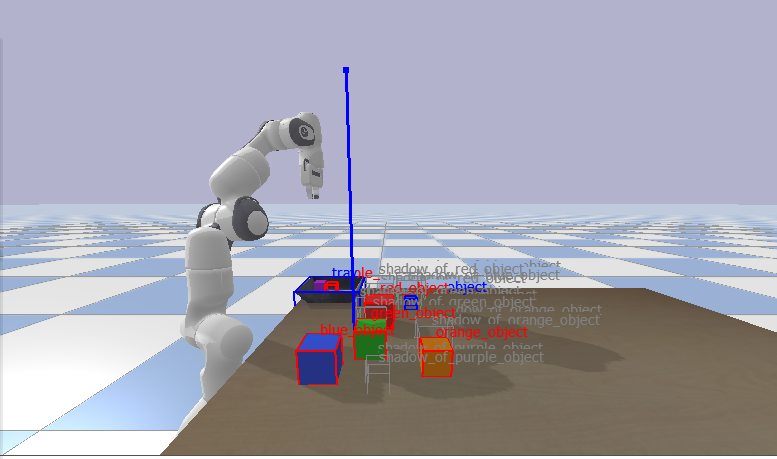
\includegraphics[width=0.85\textwidth]{sim/sense_fail_retry3.png}
    \caption{The bounded give-up in action. The log line ``retry 3/3'' marks the third consecutive still-blocked sensing attempt on a shadow; at this point the loop marks the shadow empty and proceeds, even though it was never directly observed. This is the unsound shortcut discussed above.}
    \label{fig:retry-giveup}
\end{figure}

\paragraph{Parameters.} Several geometric constants --- grasp height
offsets, approach and lift heights, the octree's minimum leaf size, the
camera pose --- are tuned for the specific table, robot, and object set
used here and would not transfer unchanged to a different setup.
Generalizing them, for example by deriving grasp parameters from object
geometry, is orthogonal to the core contribution and is noted as future
work.

\paragraph{Simplifications disclosed in the approach.} Two further
simplifications are stated where they are introduced rather than here. The
conceptual belief model uses two Know-If literals, $K(p)$ and $K(\neg p)$;
the implemented domain collapses these into a single Know-If fluent paired
with a value-carrying fluent, an equivalent encoding for the scenarios
studied (\cref{sec:kif_belief}). The \texttt{sense} action is modeled
optimistically --- it assumes the target is found --- with reactive
replanning when execution reveals otherwise, because PDDLStream and
FastDownward do not support contingent planning (\cref{ch:methods}).

  % !TEX root = ../main.tex

\chapter{Conclusion}
\label{ch:conclusion}

This thesis presented a novel approach to Task and Motion Planning under partial observability by integrating a semantic spatial abstraction, termed Boxels, with a Partially Observable Deterministic planning framework. At the core of the methodology is adaptive semantic discretization: it partitions the workspace into Boxels, concentrating detail on the objects and occluded regions that matter for the task. By modeling belief states over these Boxels, our system lets a PDDLStream-based TAMP framework plan around uncertain object locations and occlusions.

The Semantic POD-TAMP model formalizes this integration, enabling the planner to generate and execute plans that interleave information-gathering and manipulation actions. The use of K-literals to represent knowledge within the PDDL state allows for a direct and conceptually simple integration with existing POD planners. As demonstrated, this enables the robot to reason about what it knows and where uncertainty lies, and to take actions to resolve that uncertainty in a targeted manner.

This work contributes a representation in which occlusion is first-class symbolic state, letting a TAMP framework handle partial observability without enumerating an exhaustive state space and without the sub-symbolic visibility grid of a POMDP-based TAMP baseline such as TAMPURA's \emph{Find Die} benchmark. The evaluation isolates this representation by ablation---the same planner on the adaptive partition against a uniform grid at the same cell scale---and shows on three tabletop goals that it produces an order of magnitude fewer cells, lowering per-call planning time accordingly and solving find-and-tray-stack scenes that the uniform baseline effectively cannot (39.8\,\% vs 1.3\,\% success). The semantic+mbs0.05 variant---forcing a 5\,cm floor on the free-space leaf size---is indistinguishable from the default in the regime tested, indicating that placement is bottlenecked on object footprint rather than free-space resolution at these scene scales. Against the published TAMPURA POMDP-based framework, on the \texttt{holding} task --- the closest analogue to TAMPURA's \emph{Find Die} --- our planner plans in a mean 7.8\,s against TAMPURA's planning-only 57\,s, though it succeeds less often (42\,\% vs an inferred $\geq$\,63\,\%); the comparison is architectural rather than a hardware benchmark, since the difference reflects the planning machinery: TAMPURA learns and solves a probabilistic sparse MDP each step, while our deterministic knowledge-literal planner relies on replanning. The remaining directions for extending this work are outlined below.

\section{Future Work}
\label{sec:future_work}

The simplifications consolidated in \cref{sec:limitations} each suggest a
concrete next step. The following directions would extend the system beyond
the tabletop scenes evaluated here without altering its core architecture.

\paragraph{Learned perception.} The most direct extension is to replace the
oracle detector with a learned perception module that operates on the
rendered RGB-D images rather than ground-truth simulator poses. Because the
oracle is confined behind a narrow detection interface, such a module could
be substituted without changing the Boxel discretization or the planning
layer, turning the architecture's perception-agnosticism from a claim into
a demonstrated property.

\paragraph{Active sensing with a robot-mounted camera.} The current fixed
overhead camera observes the whole table at once. A robot-mounted sensor
would require the planner to reason about \emph{where to look}: a
sensing-configuration stream that computes a robot pose from which a target
region becomes visible, integrated as an additional precondition on the
\texttt{sense} action. This is the prerequisite for scenes with occlusions
not visible from any single fixed viewpoint.

\paragraph{Discovering objects beyond anticipated shadows.} When the robot
senses a shadow region, any object hidden there is discovered and added to
the representation. The scenes studied here are arranged so that every
place an object can hide is one such anticipated shadow region. Extending
the approach to objects hidden inside concave geometry --- such as a
container or cupboard, whose interior is itself a hidden region that may
hold further objects and occlusions --- would require the partitioning to
recurse: re-running over the newly revealed interior and recursively
bounding whatever it exposes.

\paragraph{Full semantic free-space merge.} Free-space cells are presently
merged only across exactly aligned shared faces. A full semantic merge that
also matches view-blocking, observability, and back-to-front ordering would
yield a coarser, more task-relevant partition with fewer Boxels, reducing
the planner's initial-state size.


  \appendix
  % !TEX root = ../main.tex

\chapter{PDDL Specification}
\label{ch:appendix-pddl}

This appendix lists the complete PDDL domain and stream definitions used by
the PDDLStream planner throughout the thesis. The domain
(\cref{sec:appendix-domain}) declares the predicates, derived predicates,
and the five actions \texttt{sense}, \texttt{move}, \texttt{pick},
\texttt{place}, and \texttt{stack}. The streams (\cref{sec:appendix-streams})
declare the four samplers that PDDLStream invokes lazily during search:
\texttt{sample-grasp}, \texttt{plan-motion}, \texttt{compute-kin}, and
\texttt{compute-stack-kin}.

\section{Domain}
\label{sec:appendix-domain}

\lstinputlisting[style=PDDL,caption={The Boxel TAMP domain.},label={lst:appendix-domain}]{resources/pddl/domain.pddl}

\section{Streams}
\label{sec:appendix-streams}

\lstinputlisting[style=PDDL,caption={Stream definitions.},label={lst:appendix-streams}]{resources/pddl/stream.pddl}


  \backmatter
  \listacronyms
  \listsymbols
  \listfigures
  \listtables
  \listalgorithms
  \listlistings
  \listreferences
  \listtodos

\end{document}
